\documentclass{jss}
\linespread{1.5}
\usepackage[round]{natbib}
\usepackage{amssymb, amsmath}
\usepackage{url, tikz}
\usepackage{hyperref}
\usepackage[sc]{mathpazo}
\usepackage[T1]{fontenc}
\usepackage{geometry}
\geometry{verbose,tmargin=2.5cm,bmargin=2.5cm,lmargin=2.5cm,rmargin=2.5cm}
\setcounter{secnumdepth}{2}
\setcounter{tocdepth}{2}
\usepackage{url}
\usepackage[utf8]{inputenc}
\usepackage{float} 
\usepackage[nottoc]{tocbibind}
\usepackage{tabularx}


%%%%%%%%%%%%%%%%%%%%%%%%%%%%%%
%% declarations for jss.cls %%%%%%%%%%%%%%%%%%%%%%%%%%%%%%%%%%%%%%%%%%
%%%%%%%%%%%%%%%%%%%%%%%%%%%%%%

%% almost as usual
\author{
\fontsize{12pt}{14.4} \textbf{Heidi Chen} \hspace{10pt} 
\fontsize{12pt}{14.4} \textbf{Yuanchu Dang} \hspace{10pt} 
\fontsize{12pt}{14.4} \textbf{David Kane} \hspace{10pt} 
\fontsize{12pt}{14.4} \textbf{Yang Lu} \hspace{10pt} 
\\ 
\fontsize{12pt}{14.4} \textbf{Kanishka Malik} \hspace{10pt} 
\fontsize{12pt}{14.4} \textbf{Skylar Smith} \hspace{10pt} 
\fontsize{12pt}{14.4} \textbf{Zijie Zhu} \hspace{10pt} }
\title{Credit Default Swaps with R}

%% for pretty printing and a nice hypersummary also set:
\Plainauthor{Achim Zeileis, Second Author} %% comma-separated
\Plaintitle{Credit Default Swaps with R} %% without formatting
\Shorttitle{Credit Default Swaps with R} %% a short title (if necessary)

%% an abstract and keywords
\Abstract{
 A credit default swap (CDS) is a bilateral agreement between two parties (the protection buyer and the protection seller) with respect to default by a third party. Over the past two decades, CDS have been one of the fastest growing parts of the financial market. First, we explain the basics of CDS along with key concepts like coupon, spread, notional, recovery rate, upfront, probability of default and the ISDA Standard Model. Second, we introduce Markit and Bloomberg, the two primary sources for CDS data and analysis. Third, we describe the CDS R package, an open source tool which allows users to calculate credit default swap information.
}
\Keywords{credit default swap, pricing, {\bf R} package}
\Plainkeywords{credit default swap, pricing, {\bf R} package} %% without formatting
%% at least one keyword must be supplied

%% publication information
%% NOTE: Typically, this can be left commented and will be filled out by the technical editor
%% \Volume{50}
%% \Issue{9}
%% \Month{June}
%% \Year{2012}
%% \Submitdate{2012-06-04}
%% \Acceptdate{2012-06-04}

%% The address of (at least) one author should be given
%% in the following format:
\Address{

  David Kane\\
  Hutchin Hill Capital\\
  E-mail: \email{dave.kane@gmail.com}

  Yuanchu Dang\\
  Department of Mathematics and Statistics\\
  Williams College\\
  1136 Paresky Center, Williamstown, MA 01267, USA\\
  Telephone: +1/413/346-7821
  E-mail: \email{Yuanchu.Dang@williams.edu}
  
  Zijie Zhu\\
  Department of Computer Science and Department of Statistics\\
  Williams College\\
  3162 Paresky Center, Williamstown, MA 01267, USA\\
  Telephone: +1/413/329-9960
  E-mail: \email{Zijie.Zhu@williams.edu}
}
%% It is also possible to add a telephone and fax number
%% before the e-mail in the following format:
%% Telephone: +43/512/507-7103
%% Fax: +43/512/507-2851

%% for those who use Sweave please include the following line (with % symbols):
%% need no \usepackage{Sweave.sty}

%% end of declarations %%%%%%%%%%%%%%%%%%%%%%%%%%%%%%%%%%%%%%%%%%%%%%%


\begin{document}



\section{Introduction}
\label{sec:Introduction}

%% Introduction should have three paragraphs, mimicing the three sentences above that give the first, second, and third goal of the paper. Each paragraph expands the details for that sentence. It is here that we mention, at least once, the 5 to 10 key bolded terms like spread, upfront, risk-neutral and so on.

This paper explains the mechanics of credit default swaps (CDS), a type of \textbf{credit derivative} that transfers \textbf{credit risk} from one group of investors to another, in exchange for payment. First, we introduces the concept of CDS with an analogy to housing insurance, and highlights that a CDS allows one party to purchase insurance (called ``protection'') on a certain investment from another party. We then introduce some simplified examples of one-period and two-period CDS in which a portfolio manager passes on risk to J.P. Morgan. Many important concepts are introduced, such as \textbf{notional amount}, \textbf{coupon}, \textbf{spread}. We also gradually introduce complications that alter CDS pricing calculations, such as \textbf{interest rates}, \textbf{recovery rate}, \textbf{probability of default}, \textbf{accrued coupon}, and \textbf{upfront payment}. In the two-period CDS example, we also introduce complications such as non-constant probability of defaults and non-constant interest rates. Then we will look at the N-period CDS as a more accurate model of real transactions. Further complications such as calculus for the continuous case will be introduced, as a culmination for this theoretical section.
  
The second section focuses on real world data from Bloomberg and Markit CDS Calculator and applies these concepts to price CDS. Bloomberg and Markit are two sources that investors can use to determine what kinds of CDS agreements they may want to make. For Bloomberg, we will dive into the specifics of Deal Section, Calculator Section and Market Section to see how theoretical concepts about CDS are translated into different indicators on the screenshot and thereby reinforce our understanding of them. Likewise, Markit CDS Calculator will be taught, with an emphasis on the terminology differences from Bloomberg, as well as useful CDS indices.

Third, we will introduce the CDS package, which allows users to calculate information regarding a particular CDS with R. The CDS package uses the same ISDA Standard Model that Bloomberg and Markit CDS Calculator use, and provide generic methods to show the calculation results in a way that is similar to Bloomberg and Markit Calculator. We also introduce some key functions which users are likely to call individually.

\section{CDS Basics}
\label{sec:CDSBasics}

\subsection{An Example: Property Insurance}
\label{sec:PropInsurance}

%% No need to have labels unless those labels are used.

Consider a simpler form of purchasing protection: property insurance. 

Suppose that a homeowner wants to purchase \$100,000 worth of property insurance on her house, covering the period from January 1 through December 31. For one year of coverage, an insurance company charges a fee of \$1,000. Call this \$1,000 the \textbf{premium}. In exchange for the premium, the insurance company agrees to pay \$100,000 to the homeowner if there is any property damage during that year. If damage does not occur, then the insurance company pockets the \$1,000 premium and doesn't pay anything to the homeowner. 

In this simplified insurance agreement, the homeowner pays the premium on January 1, the beginning of the coverage period. If the property is damaged, the insurance company pays the \$100,000 on December 31, regardless of when the damage occured. The interest rate is 0\%.

The \textbf{expected cash flows} for the agreement depend on the probability of property damage. Since the homeowner will pay the \$1,000 premium and will potentially receive \$100,000---if the house gets damaged---the homeowner's expected cash flows are as follows. ($P_h$ refers to the homeowner's estimate of probability of the property damage.)

\begin{equation}
 \begin{aligned}
   {\rm Homeowner's\hspace{3pt}expected\hspace{3pt}cash\hspace{3pt}flows = -\hspace{3pt}\$1,000 + (P_h \times {\$100,000})}
    \end{aligned}
    \label{eqn:homeownerECF}
\end{equation}

Since the insurance company will receive the \$1,000 premium and will potentially pay \$100,000---if the house gets damaged---the insurance company's expected cash flows are as follows. ($P_c$ refers to the insurance company's estimate of the probability of property damage.)

\begin{equation}
 \begin{aligned}
   {\rm Insurance\hspace{3pt}company's\hspace{3pt}expected\hspace{3pt}cash\hspace{3pt}flows = \hspace{3pt}\$1,000 - (P_c \times {\$100,000})}
    \end{aligned}
    \label{eqn:companyECF}
\end{equation}

Note that $P_h$ and $P_c$ do \emph{not} have to be the same. The homeowner and the insurance company may have two different estimates of the probability that the house will get damaged during the year. The homeowner doesn't know the insurance company's estimate, and the insurance company doesn't know the homeowner's estimate. In fact, an outside third party does not know either $P_h$ or $P_c$. 

Assume that both the homeowner and the insurance company are \textbf{risk-neutral}, meaning that they only care about expected cash flows. For example, a risk-neutral investor would be willing to pay \$1 for a 1\% chance of a \$100 payment and would view the two sides --- the \$1 and the 1\% chance of \$100 --- as equal in value. Most investors are not risk-neutral. They would prefer a guaranteed \$1 over a 1\% chance of winning \$100. Assumethat both parties agree to the above insurance agreement. What does this imply about $P_h$ and $P_c$? 

The homeowner only agrees to the deal if $P_h \geq 0.01$. Any lower value would mean that her expected cash flows were negative and, by assumption, we know that neither the homeowner or the insurance company will enter an agreement with negative expected cash flows. For the same reasons, if the insurance company agrees to the deal, then $P_c \leq 0.01$. Neither of these facts allow us to conclude anything about $P_true$, the true probability of damage. Either the homeowner or the insurance company or both could be wrong in their estimates. However, we can now define $P$ --- \textbf{risk-neutral estimate of the probability of property damage} --- as the single value for both $P_h$ and $P_c$ which makes the expected cash flows identical. Mathematically:

\label{eqn:PropertyInsurance}
\begin{align}
  \rm -\hspace{3pt}\$1,000 + P \times {\$100,000}  &= \rm \$1,000 - P \times {\$100,000} \\
  \rm 2 \times P \times {\$100,000}  &=  \rm 2 \times \$1,000 \\
  \rm P \times {\$100,000}  &= \rm {\$1,000} \\
  \rm P  &= \rm 0.01
\end{align}

Therefore, the risk-neutral probability of property damage is 1\%. Note that this number does not tell us anything about either $P_h$ and $P_c$. The homeowner's estimate for the probability of damage is at \emph{least} 1\% because she refuses any agreement with negative expected cash flow. For example, say the homeowner believes that there is a 1.5\% chance that the house will be damaged. She would want to make a deal in which the risk-neutral probability of damage was 1\% because her expected cash flows are positive.  The same analysis applies to the insurance company. 

Clearly, 1\%---the risk neutral probability of property damage---is a very important value for this agreement. We need to note, however, that this value is not necessarily the \emph{true} probability of property damage, nor are the parties' predictions for the probability of damage. Consider an extreme example: what if, as the two parties initiate the agreement, an asteriod sets on a course to crash into the house in six months. In such a case, the probability of damage is 100\%. However, neither party has forseen this occurence, so the risk-neutral value of $P$ (1\%) and the parties' predictions of $P$ (1.5\% and 0.5\%) are certainly not equal to the true value of $P$ (100\%).

\subsubsection{Property Insurance Complications}
\label{sec:PIComplications}

Unfortunately, the above insurance purchase---although relatively simple---made several assumptions that excluded real aspects of the insurance market. Some of these aspects are parallel to aspects in the CDS market that we will assume and exclude from calculations in all sections of this paper. Below we list such assumptions:

1. We assumed that the homeowner was risk-neutral when, in reality, homeowners who purchase property insurance are generally risk-adverse. Since they want to avoid risk, they view the process of purchasing insurance as more of a necessity than an option. They are willing to pay more (i.e. a larger coupon payment) than required for the expected cash flows to be equal. Taking our example, if the homeowner is risk-adverse and believes the probability of damage to be 1.5\%, she would be willing to pay a coupon of more than 1.5\%.

2. We assumed that both parties would only concede to the insurance agreement if the expected cash flows were equal. As the above assumption demonstrated, an insurance buyer is generally willing to have a smaller expected cash flow than the insurance company. Conversely, insurance companies need to have higher expected cash flows than their clients (the insurance buyers) because they aim to \emph{profit} from selling insurance; if they charge as much as they expect to pay, then they can't expect to make any money as a company. 

3. We discussed the insurance agreement in a way that assumed we knew if there had been damage. How does the insurance company determine that there has been, for example, a house fire when the homeowner claims that one occured? The insurance company would probably want some form of proof, and the company might even have someone visit the house and confirm the damage. 

While the above assumptions represent assumptions that we will maintain throughout the paper, the following assumptions are one that this paper will, in fact, account for in parallel situations regarding CDS. We list them below:

1. The insurance agreement assumed that any damage would merit the insurance payment of \$100,000. However, what if, for example, the toaster caught on fire and damaged only the toaster? What types of \textbf{events} does the insurance company define as ``damage''? These questions highlight the importance of a detailed insurance contract that specifies these terms.

2. The agreement considered only the following two cases: either the entire house was damaged (and the insurance company paid \$100,000), or the house was not damaged (and the insurance company paid \$0). However, there are other likely outcomes we need to account for. For example, what if only half of the house was damaged? In that case, it would not make sense for the insurance company to pay \$100,000; instead, the company should compensate only for the damaged section of the house by paying \$50,000. 

3. We stated in the beginning of the property insurance example that the interest rate was 0\%. Clearly, this is not the case in the insurance market, so we would need to account for that change in our calculations which we'll discuss later.

4. We largely simplified the insurance agreement by creating a one-year agreement from January 1 to December 31. This, too, does not have to be the case in the insurance market. The agreement could be longer or shorter than a year and does not need to fit neatly within a calendar year.

5. The insurance agreement included one premium payment of \$1,000. However, there are cases in the insurance market where there are multiple premium payments on different dates. We did not account for that possibility in our example, but we will account for parallel situations in the CDS market.

\subsection{Simple One-Period CDS}
\label{sec:OnePeriod}

Instead of buying insurance against property damage, consider buying insurance against a company's inability to pay back its bondholders. The risk of a company being unable to meet its debt obligations is known as \textbf{credit risk}. In Figure \ref{fig:AlcoaBond} below, we can see details of a bond of Alcoa Inc. If we look to the right of the figure, under ``Bond Ratings,'' we can see certain symbols representing \textbf{credit ratings} that are provided by rating agencies such as Moody's, S\&P and Fitch. These symbols are indicators of a company's credit risk. We will not go into the details of how these ratings are determined, since those details are beyond the scope of this paper. What we should note is that companies that have credit ratings of BBB- or higher from S\&P or Fitch or Baa3 or higher from Moody's can be classified as \textbf{Investment Grade} (IG) bonds. Naturally, if a company's credit risk goes up, investors would demand a higher yield and consequently, a lower price. If a company is very likely to meet its debt obligations---or if it has consistently done so in the past---the company can be known as \textbf{credit worthy}.

\begin{figure}[H]
\centering
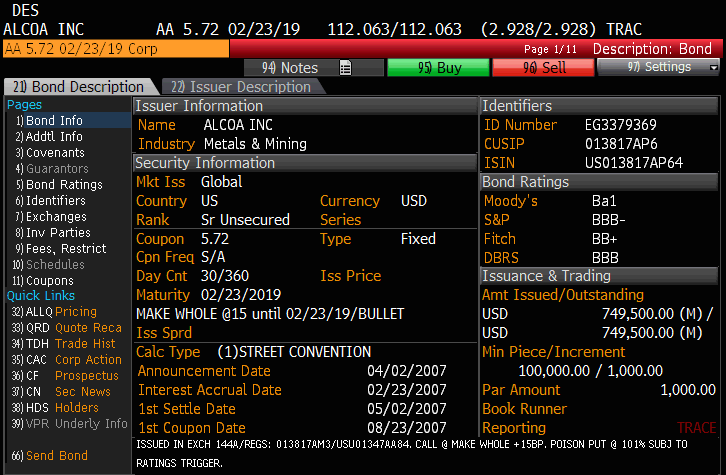
\includegraphics[width=5in, height=3.7in]{images/AlcoaBond.png}
\caption{Bloomberg data taken on June 24, 2014 for senior Alcoa bonds that will mature on February 23, 2019. These bonds have a duration of twelve years, since the bonds were initiated on April 2, 2007 (see ``Announcement Date''). This figure displays essential information regarding the bonds that a potential investor would need to consider, such as the company (``name''), industry, seniority (``rank''), the value of the coupon payments (``coupon''), maturity, coupon payment dates and credit ratings. (Many of these attributes and concepts will be further discussed in Section \ref{sec:BloombergMarkit}.)}
\label{fig:AlcoaBond}
\end{figure}

CDS are used for the purpose of hedging against the \textbf{credit risk} associated with bonds. Let's say a portfolio manager at a hedge fund, Citadel, believes that Alcoa, isn't likely to return the money that its bondholders have lent it. In other words, she believes that Alcoa will \textbf{default} on its bonds---not pay them back. She enters a one-year CDS agreement with an investment bank---say, J.P. Morgan (JPM)\footnote{For ease of reading, we desginate the buyers of protection in our examples as female and the sellers of protection as male.}---in which she purchases protection of \$100,000, an amount known as the \textbf{notional amount} of the CDS. Note that bondholders can purchase protection on their bonds (i.e. an Alcoa bondholder can enter a CDS in which she purchases protection against Alcoa's default), but this does not have to be the case. In our example, the portfolio manager does not own Alcoa bonds. 

Keep the same timeline (January 1 to December 31) and numerical figures from our property insurance example. The interest rate is still 0\%. In exchange for protection on the \$100,000, the portfolio manager agrees to pay a \textbf{coupon} (equivalent to the premium in our property insurance example but different terminology) of 1\% of the notional amount. The coupon payment of \$1,000 is paid on January 1, the beginning of the coverage period. This side of the CDS is called the \textbf{premium leg}, and the portfolio manager is known as the \textbf{protection buyer}, since she is purchasing protection.

The other side of the CDS agreement is known as the \textbf{protection leg}, since it involves protection payment in case of default, and involves JPM, called the \textbf{protection seller}. If Alcoa defaults, JPM pays the notional amount of \$100,000 to the portfolio manager on December 31, the end of the coverage period. Alcoa is known as the \textbf{reference entity} in this CDS since the protection buyer desires protection for Alcoa. 

Note that we are using the terms "premium" and "coupon" synonymously. Premium is commonly used to describe the periodic fee paid by the protection buyer, which is why this side of a CDS is called the premium leg. However, even though the coupon is commonly used to describe the periodic fee paid to a bondholder, coupon can also be used to describe the periodic fee in a CDS context. For clarity, we will just use coupon in this paper when referring to the periodic fee paid by the protection buyer.

Since the portfolio manager makes money if Alcoa deteriorates, she can be said to be \textbf{short} credit. Shorting is generally a method of profiting from the deterioration of a security, such as a bond. Alternatively, since JPM loses money if Alcoa collapses, JPM can be said to be \textbf{long} credit. In other words, JPM's returns are similar to those of a person who owns Alcoa bonds. If Alcoa does well, JPM does well, and if Alcoa doesn't, then JPM doesn't either.

The expected cash flows for the agreement depend on the probability of default. Since the portfolio manager will pay the \$1,000 premium and will potentially receive \$100,000 if Alcoa defaults, the portfolio manager's expected cash flows---which represent the premium leg---are as follows. (the below $P$ refers to the portfolio manager’s prediction of probability of default.)

\begin{equation}
 \begin{aligned}
   {\rm Portfolio\hspace{3pt}manager's\hspace{3pt}expected\hspace{3pt}cash\hspace{3pt}flows = -\hspace{3pt}\$1,000 + (P \times {\$100,000})}
    \end{aligned}
    \label{eqn:portfolioECF}
\end{equation}

Since JPM will receive the \$1,000 premium and will potentially pay \$100,000 if Alcoa defaults, JPM's expected cash flows---which represent the protection leg---are as follows. (the below $P$ refers to JPM’s prediction of probability of default.)

\begin{equation}
 \begin{aligned}
   {\rm JPM's\hspace{3pt}expected\hspace{3pt}cash\hspace{3pt}flows = \hspace{3pt}\$1,000 - (P \times {\$100,000})}
    \end{aligned}
    \label{eqn:jpmECF}
\end{equation}

Note that the portfolio manager's expected cash flows are the same as that of the homeowner in the property insurance example, and JPM's expected cash flows are the same as that of the insurance company. This shouldn't be too surprising, though, since the numerical figures in both examples are the same.

We will again assume that both parties in the CDS are risk-neutral and that both parties will only enter deals in which the expected cash flows are equal.

Consider that a deal is reached: both parties agree to the CDS. As in the property insurance example, we can equate the cash flows to find the \textbf{risk-neutral probability of default}, which is the value of $P$ implied by the deal. Note that an alternate definition of this probability is the value of $P$ at which the premium leg equals the protection leg:

\label{eqn:SimpleOnePeriod}
\begin{align}
   \rm Portfolio\hspace{3pt}manager's\hspace{3pt}expected\hspace{3pt}cash\hspace{3pt}flows &= \rm JPM's\hspace{3  pt}expected\hspace{3pt}cash\hspace{3pt}flows \\
   \rm Premium\hspace{3pt}leg &= \rm Protection\hspace{3pt}leg \\
   \rm -\hspace{3pt}C + (P \times V)  &= \rm C - (P \times V)
\end{align}

The left side of Equation \ref{eqn:SimpleOnePeriod} indicates that the portfolio manager has to pay the coupon, $C$, but could receive the protection leg of $V$, depending on $P$. The right indicates the converse: JPM will receive the coupon payment, $C$, but could potentially have to pay the protection leg of $V$, depending on $P$.
Plugging in known values ($C$ = \$1,000 and $V$ = \$100,000), we get:

\begin{equation}
 \begin{aligned}
   {\rm -\hspace{3pt}\$1,000 + (P \times {\$100,000})  = \$1,000 - (P \times {\$100,000})}
    \end{aligned}
\end{equation}

Since this is the same equation and the same numerical figures from the property insurance example, we know that P = 1\%. Note that this 1\% only represents the ``risk-neutral'' value of $P$. Generally speaking, ``risk neutral'' means that one is indifferent regarding the choice between, say, (A) \$100 for sure and (B) an offer of being equally likely to receive \$50 or \$150. In other words, it implies no additional premium for taking on risks, or, equivalently, a Sharpe ratio of $0$. Therefore, it does not indicate the values of $P$ that the two parties believe to be true, nor does it indicate the true value of $P$. Parallel to the property insurance example, we can infer (given both parties have agreed to the CDS) that the portfolio manager's prediction of $P$ must be at least 1\%, and JPM's prediction of $P$ must be at most 1\%. In fact, from here on out, when we mention the risk-neutral probability of default for a CDS example, we can take this to mean that the protection buyer's prediction of $P$ is at least the risk-neutral value, and the protection seller's prediction of $P$ is at most that risk-neutral value.

We will call the above CDS example the simple one-period CDS.

\subsubsection{One-Period Case Over Time}
\label{sec:OnePeriodOverTime}

In order to fully understand the nature of a CDS, we should look at what happens to the simple one-period CDS over the life of its contract---specifically, how the risk-neutral probability of default (or risk-neutral $P$), the \textbf{mark-to-market} value, the \textbf{spread}, and the \textbf{profits and losses} (P&L) of the Citadel portfolio manager and JPM change from January 1 to December 31, assuming that Alcoa does not default during that year.

We can think of the mark-to-market value as the price at which the CDS would sell at any given time over the life of the contract. For example, on June 30, midway through the year, a prospective buyer would pay \$500 to the portfolio manager in order to replace her as the protection buyer. Since the portfolio manager pays the \$1,000 coupon payment on Janaury 1 and would recieve \$500 from the prospective buyer on June 30, both the portfolio manager and prospective buyer pay a net amount of \$500---which makes sense since one year of coverage merits a coupon payment of \$1,000 and thus six months of coverage merits \$500. 

We can consider the spread to be equal to the coupon in this particular CDS (we will discuss the spread in more detail in the section regarding non-standard coupon). A different is that we refer to coupons in percentages---in this case, 1\%---and we refer to spreads in basis points (bps). 1\% is equal to 100 bps.

P&L represents the change in market value of the CDS contract on, in this case, a day to day basis. A good way of thinking about the P&L of, for example, JPM in this CDS is to consider the fraction of the coupon payment that JPM \emph{earns} each day. We know that JPM recieves a coupon payment of \$1,000 on January 1, but JPM's P&L measures what JPM earns each day that it provides protection during that year.

Here is a table that considers what happens to the above-mentioned variables as the contract matures from January 1 to December 31. Note that we are considering the case in which Alcoa does not default during the one-year contract.

\begin{table}[H]
\centering
{\footnotesize
\begin{tabular}{llllllll}
  \hline
Date & Cash flows (Citadel) & Cash flows (JPM) & Risk-neutral $P$ & Mark-to-market & Spread & P&L (Citadel) & P&L (JPM) \\ 
  \hline
  Jan 1 & -\$1,000 & \$1,000 & 1\% & \$1,000 & 100 bps & \$0 & \$0 \\ 
  Mar 31 & \$0 & \$0 & .75\% & \$750 & 75 bps & -\$250 & \$250 \\ 
  Jun 30 & \$0 & \$0 & .50\% & \$500 & 50 bps & -\$500 & \$500 \\ 
  Dec 31 & \$0 & \$0 & 0\% & \$0 & 0 bps & -\$1,000 & \$1,000 \\
   \hline
\end{tabular}
}

\caption{This table measures how several variables---the cash flows for each party, the risk-neutral value of $P$, the mark-to-market value of the contract, the spread, and the P&L for each party---change as the simple one-period CDS matures. Since this table considers the case in which the reference entity---Alcoa---does not default, the only cash flow is the \$1,000 coupon payment from the Citadel portfolio manager to JPM on January 1. The risk-neutral value of $P$ decreases from 1\% to 0\% as the contract matures. Please notice that this ``linear'' drop of the risk-neutral $P$ which is proportional to the time remaining the termination of the contract is a simplified model, whose complication we will discuss later in this section. The mark-to-market value decreases from \$1,000 to \$0 from January 1 to December 31 and the spread decreases from 100 bps to 0 bps. Note that as JPM profits from providing protection coverage (gains \$1,000 by Dec 31), the portfolio manager loses. On January 1, the P&L of both parties is 0.} 
\label{table.1}
\end{table}

As we can see in Table \ref{table.1}, the risk-neutral $P$ decreases from 1\% on January 1 to 0\% on December 31. On June 30, the risk-neutral $P$ has dropped to 0.5\% because only half of a year remains for Alcoa to default during the contract---and thus the risk-neutral $P$ is half of its initial value. This demonstrates the direct relationship between the risk-neutral $P$ and the contract duration. 

In our simple one-period case, we say that the coupon is 1\% and the spread is 100 bps. We can observe in Table \ref{table.1} that the spread decreases from 100 bps to 0 bps over the year---a reflection of the fact that, at the end of the contract, JPM has earned and been paid the full \$1,000 coupon payment by providing a full year of coverage. This process---the spread drop over the duration of the contract---is known as \textbf{rolling down the curve}. 

\subsubsection{Simple One-Period Case Complications}
\label{OnePeriodComp}

Similar to the property insurance example, we made several assumptions in our simple one-period CDS that are not consistent with the CDS market. 

1. Similar to the property insurance example, we assumed that the protection buyer was risk-neutral, when she could very well be risk-adverse. She may be willing to pay a coupon larger than 1\% even if she predicts the probability of default to be 1\% because she strongly desires to have protection on Alcoa.

2. Also like the property insurance example, we assumed that both parties would only agree to the deal if the expected cash flows were equal. This could very well not be the case if, for example, JPM is selling protection in many CDS agreements and needs or wants to make a profit.

3. In the simple one-period CDS, we assumed that the protection leg would only be paid out in the case of default and bankruptcy. However, depending on the particular CDS, the protection leg could be paid out even if the reference entity defaults and doesn't go bankrupt. In fact, there are several scenarios that can be considered \textbf{credit events}---occurences that merit the payout of the protection leg in a CDS. Besides default and bankruptcy, common credit events include failure to return money to bondholders within a certain amount of time, a credit rating downgrade (explained in Section \ref{sec:BloombergMarkit}) and the confiscation of assets, among other events.

Because we made many more assumptions and failed to address many aspects of a CDS, we have split up the following simple one-period CDs complications into five separate sections that address interest rate, recovery rate, accrued coupon, non-standard coupon and upfront payment. 

\subsubsection{Interest Rates}
\label{sec:InterestRate}

Up until now, we have assumed that the interest rate is 0\% in the simple one-period CDS. The \textbf{interest rate} is a benchmark rate that participants in the CDS market use to discount cash flows. How might the cash flows in the CDS agreement change if the interest rate was \emph{not} 0\%?

First, look at our CDS agreement: the portfolio manager pays the premium on January 1 and JPM pays the \$100,000 (if Alcoa defaults) on December 31. JPM receives the \$1,000 coupon a full \emph{year} before the portfolio manager would receive the \$100,000 payment if Alcoa defaults. In an environment where the interest rate is 10\%, JPM could theoretically invest the \$1,000 sum starting January 1 and earn interest for that year:

\begin{equation}
 \begin{aligned}
  {\rm Coupon\hspace{3pt}with\hspace{3pt}Interest = {\$1,000}\times{(1 + .10)} = \$1,100} 
    \end{aligned}
\end{equation}

Not just coupon grows at the interest rate. Similar discounting effect applies to potential credit loss as well. If a credit event triggers a loss in the future, then we must discount the loss amount by a proper effective interest rate $i$ to get the present value, before we can set up the equality and solve for the risk-neutral $P$.

Here are the expected cash flows for a generic case. ($P$ refers to the risk-neutral probability of default; $V$ represents the notional value; $i$ stands for the interest rate; and $C$ is the coupon payment).

\begin{equation}
 \begin{aligned}
  {\rm -\hspace{3pt}C} + \frac{P \times V}{(1 + i)} = C - \frac{P \times V}{(1 + i)} 
    \end{aligned}
\label{eqn:InterestRate}
\end{equation}

How might a discounted credit loss affect $P$, the risk-neutral probability of default which, by definition, equates the expected cash flows? Plugging in known values:
\begin{equation}
 \begin{aligned}
  {\rm -\hspace{3pt}\$1,000 + \frac{P \times \$100,000}{(1 + 0.1)} = \$1,000} - \frac{P \times \$100,000}{(1 + 0.1)} 
    \end{aligned}
\end{equation}

Solving for $P$, we get 1.1\%. Since both parties agreed to this CDS in an environment where the interest rate is 10\%, we can say that the portfolio manager's prediction for the probability of default is at least 1.1\%, and JPM's prediction for the probability of default is at most 1.1\%. 

\subsubsection{Recovery Rate}
\label{sec:recovery}

Recall that in our property insurance example, we mentioned that some cases---such as a house fire that burns half of a house---may not merit a full payment equal to the notional amount (in that case, \$100,000). Similarly, when a company defaults, an \textbf{auction} occurs in which some of the company's bondholders come to sell their bonds, and prospective buyers come to buy the bonds at, usually, lower prices. We note this because the price at which bonds can be sold after default affects the protection leg payment in a CDS contract.

Suppose that Alcoa defaults during the simple-one period CDS, and a bond that had a face value of \$100 can now be sold at the auction for a price of \$55. (Note for each complication in the simple one-period CDS, we are ignoring the effects of the other complications. For example, we assume that that there is an interest rate of 0\% in this example.)

In this case, the \textbf{recovery rate}---the rate representing the amount of value a bond retains after default---is 55\%. As such, JPM would only have to pay 45\% of the notional amount---\$45,000---instead of the notional amount of \$100,000 because bondholders who have purchased protection are able to retain 55\% of their bonds' worth. 

So, we need to factor the recovery rate into our calculation of expected cash flows because it changes the value of the protection leg in the simple one-period CDS. Since the portfolio manager and JPM will only both agree to this CDS if the expected cash flows are equal, we set the portfolio manager's expected cash flows and JPM's expected cash flows equal to each other. ($RR$ refers to the recovery rate and, as before, $P$ is the risk-neutral probability of default, $C$ is the coupon payment, and $V$ is the notional value.)

\label{eqn:recovery}
\begin{align}
  \rm Portfolio\hspace{3pt}manager's\hspace{3pt}expected\hspace{3pt}cash\hspace{3pt}flows &= \rm JPM's\hspace{3pt}expected\hspace{3pt}cash\hspace{3pt}flows \\
  \rm - C + (P \times V \times (1 - RR)) &= C - (P \times V \times (1 - RR))
\end{align}

Note that the above equation is an extension of Equation \ref{eqn:SimpleOnePeriod}, the only difference being that we mupltipled $V$ by (1 - RR) to account for the change in the protection leg. The protection seller only has to pay the fraction of the notional amount that the recovery rate does \emph{not} account for (hence (1 - RR) instead of just $RR$). Another term for this amount is the loss given default (LGD):

\begin{equation}
 \begin{aligned}
   {\rm (1 - RR) = LGD}
    \end{aligned}
\label{eqn:recovery}
\end{equation}

We'll stick to using $RR$ instead of the LGD for now.

To solve for the risk-neutral probability of default, we plug in known values ($C$ = \$1,000, $V$ = \$100,000, and $RR$ = 0.55)

\begin{equation}
 \begin{aligned}
   {\rm - \$1,000 + (P \times \$100,000 \times (1 - 0.55)) = \$1,000 - (P \times \$100,000 \times (1 - 0.55))}
    \end{aligned}
\end{equation}
After combining like terms, dividing both sides by 2 and simplifying, we get:
\begin{equation}
 \begin{aligned}
   {\rm P \times \$55,000 = \$1,000}
    \end{aligned}
\end{equation}

Therefore, $P$ is 1.8\% (rounded to the nearest tenth) in this scenario where the recovery rate is 55\%.

\subsubsection{In the Case of a Default}
\label{sec:SettlementType}

When a default does occur, the protection seller would owe the protection buyer the notional amount minus any money recovered from the company. It must be noted that the protection is effective for the credit events that have taken place since 60 days \textit{before} the trade date; this date is known as the \textbf{backstop date}. Before the ``Big Bang Protocol'' in April 2009, this date used to be one day \textit{after} the trade date. If there is a delay in awareness about a credit event, the new system allows sufficient time for the two dealers to discover and process the information. 

Should a bond (that is the reference obligation in a CDS agreement) default, the counterparties can compensate accordingly in two ways. The first is a \textbf{physical settlement} in which the buyer will actually deliver the defaulted bonds to seller, and the seller will then pay the face value of those bonds. The disadvantage to this particular transcation is that the buyer(s) of protection will have to find and deliver those bonds to the seller even if they don't own the bonds themselves. This may artificially drive up the price of the bonds, and is more likely to happen when there is a large number of outstanding CDS contracts. 

The alternative to a physical settlement is a \textbf{cash settlement}, in which the seller simply pays the following to the buyer: notional amount $\times$ (1 - recovery rate). Unfortunately, determining a recovery rate is often an issue. One approach the ISDA has adopted lately is an \textbf{auction} style process in which major dealers submit their bids for the value they place on a company's debt.  CDS contracts for corporate bonds generally assume a 40\% recovery rate for valuation purposes.

\subsubsection{Accrued Coupon}
\label{sec:AccruedCoupon}

Back to our simple one-period CDS example---0\% interest rate, 0\% recovery rate. For this scenario, both the premium leg and the protection leg are paid on December 31. We have so far assumed that our CDS agreement between the portfolio manager and JPM begins on January 1 and ends on December 31 of the same year. However, what if this agreement wasn't made exactly on January 1? What if it was made on March 31, one quarter through the year? Using our simple one-period CDS example, this implies that the portfolio manager would have to pay the same coupon of $1\% \times (\$1,000)$ on December 31 for only receiving nine months (instead of one year) of protection coverage.

Assume that both parties agreed to a deal under these conditions. 

Since the risk-neutral probability of default decreases as the contract duration decreases (see \ref{table.1}), the risk-neutral probability that Alcoa will default in nine months is less than the risk-neutral probability that it will default in twelve. As such, the expected cash flows are no longer equal and therefore the two parties must have accounted for this discrepancy---otherwise the portfolio manager would not have agreed to the above CDS. In other words, given that the agreement was made, JPM must have paid an additional sum to the portfolio manager to compensate for the fact that she is paying the coupon for one-year coverage and is only receiving nine months.

In order to determine this sum, we need to calculate the fraction of the coupon she is unfairly paying, or the fraction of the coupon that accounts for the first three months of the year (January 1 to March 31). This fraction of the coupon payment is known as the \textbf{accrued coupon}.

\begin{equation}
 \begin{aligned}
  {\rm Accrued = \frac{90}{360}\times\frac{1.0}{100}\times\$100,000 = \$250}
    \end{aligned}
\end{equation}

In order to determine the accrued coupon, we multiply the coupon (1\%) by the notional amount (\$100,000) to get the coupon payment (\$1,000), and then we multiply the coupon payment by the fraction of the year that the portfolio manager did not receive coverage for---in this case, 90/360 or one fourth. 

Note that we are dividing 90 by 360 instead of 365 in the above calculation. This particular CDS contract can be said to have a 30/360 \textbf{day count convention}, which means that the accrued coupon calculations are based on the assumptions that there are 30 days in a month and 360 days in a year. For example, if we are trying to find the number of days between date one, $M_1$/$D_1$/$Y_1$, and date two, $M_2$/$D_2$/$Y_2$, using the 30/360 convention, we use the following formula with exceptions listed below:

\begin{equation}
 \begin{aligned}
  {\rm Number\hspace{3pt}of\hspace{3pt}days = 360 \times (Y_{2} - Y_{1}) + 30 \times (M_{2} - M_{1}) + (D_{2} - D_{1})}
    \end{aligned}
\end{equation}

Exceptions:

1. If $D_1$ is 31, assume that $D_1$ is 30.

2. If $D_2$ is 31 and $D_1$ is 30 or 31, assume that $D_2$ is 30.

3. If $M_1$ is 2, and $D_1$ is 28 (not in a leap year) or 29, assume that $D_1$ is 30.

For example, according to this convention, if the simple one-period CDS agreement was initiated on February 28 (during a non-leap year), then we would calculate the number of days between 01/01/$Y_a$ and 02/28/$Y_a$ (where $Y_a$ is a specific year) to be 59, since we consider February 28 to be the last day in a 30-day month (according to exception 3 above):

\begin{equation}
 \begin{aligned}
  {\rm Number\hspace{3pt}of\hspace{3pt}days = 360 \times (0) + 30 \times (2 - 1) + (30 - 1) = 59}
    \end{aligned}
\end{equation}

If a CDS agreement was initiated on October 31, then we would calculate the number of days in between 01/01/$Y_a$ and 10/31/$Y_a$ (where $Y_a$ is some year) to be 300. Note that it does not matter for this calculation if $Y_a$ was a leap year or not.

\begin{equation}
 \begin{aligned}
  {\rm Number\hspace{3pt}of\hspace{3pt}days = 360 \times (0) + 30 \times (10 - 1) + (31 - 1) = 300}
    \end{aligned}
\end{equation}

The purpose of this day count convention is to make calculations easier.

Since a \$250 cash flow from JPM to the portfolio manager compensates for the amount of the coupon that the portfolio manager is unfairly paying, we can model the expected cash flows for the agreement:

\begin{equation}
 \begin{aligned}
   {\rm - \$1,000 + (P \times \$100,000) + \$250 = \$1,000 - (P \times \$100,000) - \$250}
    \end{aligned}
\end{equation}

Again, as neutral observer of the market (neither the buyer nor the seller), we are interested in how these expected cash flows affect $P$, the risk-neutral probability of default? Solving for $P$, we get:

\begin{equation}
 \begin{aligned}
   {\rm P \times \$100,000 = \$750}
    \end{aligned}
\end{equation}

Therefore, the risk-neutral probability of default in this CDS is .75\%. Note that this is different than that of the simple one-period CDS (1\%). Note that in Table \ref{table.1}, we observed that the risk-neutral probability of default decreases as the contract matures. 

In Section \ref{sec:OnePeriodOverTime}, we measured different aspects of a CDS over the life of the contract. Recall that we defined the mark-to-market value as the coupon that a prospective buyer would pay at a given time to own the protection for the remainder of the CDS. We could similarly measure the value of the accrued coupon over the life of the contract---or the accrued coupon value that JPM would have to pay a prospective buyer if she bought the protection from the portfolio manager at a given time in the contract. Consider the table below:

\begin{table}[H]
\centering
{\footnotesize
\begin{tabular}{lllll}
  \hline
Date & Mark-to-market & P&L (Citadel) & P&L (JPM) & Accrued Coupon \\ 
  \hline
  Jan 1 & \$1,000 & \$0 & \$0 & \$0\\ 
  Mar 31 & \$750 & -\$250 & \$250 & \$250\\ 
  Jun 30 & \$500 & -\$500 & \$500 & \$500\\ 
  Dec 31 & \$0 & -\$1,000 & \$1,000 & \$1,000\\
   \hline
\end{tabular}
}
\caption{This table measures the mark-to-market value, the P&L for both parties, and the accrued coupon value over the life of the contract. Note that the mark-to-market values and accrued coupon values are the same for each date. In other words, the accured coupon that accounts for the time passed is equal to the price that a prospective buyer would have to pay the portfolio manager for protection for the remainder of the CDS. The absolute value of each party's P&L is also equal to the accrued coupon value; the accrued coupon that accounts for the time passed is equal to the money the JPM has earned by providing protection for the time passed.}
\end{table}

As we can see, the accrued coupon increases as the contract matures---or, in other words, the coupon that accounts for the time in the contract that has passed \emph{increases} as the contract matures.

Note that accrued coupon only becomes relevant when the contract does not initiate on a coupon payment date. In the real-world CDS market, there are four dates each year---instead of, in our example, the one date of January 1---when coupon payments can be made. These dates are known as \textbf{roll dates} and comprise the following: March 20, June 20, September 20, and December 20. As we proceed with our simple CDS example, however, we'll continue with the assumption that January 1 is the one and only ``roll date.''  

There is also another related but different concept called accrued payment, which is paid by the protection buyer to the protection seller once a credit event happens. This payment is meant for the protection received between the last coupon date and the event date, since credit events might well not happen on a coupon date.

Both these ``accrued'' amounts serve as necessary adjustment to the payment of CDS transactions.

\subsubsection{Non-standard Coupon and Big Bang Protocol}
\label{sec:nonStandardCoupon}

In all of our CDS examples, we have assumed a coupon of 1\%. We have done so because we have been working with the same basic numerical figures: a risk-neutral probability of default of 1\% and a notional amount of \$100,000:

\begin{equation}
 \begin{aligned}
   {\rm - \$1,000 + ((P = 1\%) \times \$100,000) = \$1,000 - ((P = 1\%) \times \$100,000)}
    \end{aligned}
\end{equation}

In other words, we have been considering cases in which the portfolio manager believes the probability of default to be at least 1\%, and JPM believes the probability of default to be at most 1\%. 

What if, however, the portfolio manager actually thought that the probability of default was 3\%, and JPM thought it was 4\%? The portfolio manager would want to make CDS agreements with risk-neutral probabilities of default of 3\% or greater because if it's greater then she is paying the same coupon for a higher probability that she'll receive \$100,000. JPM would want to make CDS agreements with risk-neutral probabilities of default of 4\% or smaller because if it's smaller then JPM is receiving the same coupon for a smaller probability that it'll have to pay \$100,000. The range of possible risk-neutral probabilities at which they would agree is 3\% to 4\%. Say they decide on 3\%.

In such a case, the expected cash flows would only be equal if the coupon payment was \$3,000: 3\% of the notional amount of \$100,000. As such, here is a case in which the coupon would not be 1\%:

\begin{equation}
 \begin{aligned}
   {\rm - \$3,000 + ((P = 3\%) \times \$100,000) = \$3,000 - ((P = 3\%) \times \$100,000)}
    \end{aligned}
\end{equation}

In fact, that is a simplified example of how protection buyers and sellers determined coupon payments before April, 2009. Traders could theoretically enter CDS agreements with any coupon---say, .72\% or 1.63\%---because there were not any market conventions for coupon values. Each CDS had a specific \textbf{spread}---in this context, a specific coupon---that equated the two expected cash flows in the CDS. If a person was interested in buying CDS protection, she and the protection seller would refer to different CDS agreements by simply quoting the corresponding coupons.

One issue with this system was that traders could not easily trade CDS, since each CDS had a specific coupon.
For example, investment banks like JPM often buy protection for one CDS and sell protection for another so as to offset each deal and \textbf{hedge} its risk. However, this became difficult to do when the CDS agreements had different coupons and thus different expected cash flows.

So, in 2009, a regulatory organization known as the International Swaps and Derivates Association (ISDA) 
introduced new CDS market conventions in North America which required buyers and sellers to trade at coupons of 100 bps or 500 bps. This, along with a number of other regulatory changes, came to be known as the `Big Bang Protocol`. Since then, the spread of a CDS no longer signifies the coupon at which the CDS is traded; instead, the spread is the coupon that the CDS \emph{would} be traded at in a market without standardized coupons---or the coupon that the CDS would have been traded at before 2009. In order to account for the discrepancy between the spread and the standardized coupon at which a CDS must trade, protection buyers and sellers use \textbf{upfront payments}, discussed in the next section.

\subsubsection{Upfront Payment}
\label{sec:Upfront}

An \textbf{upfront payment}---a payment made from one party to the other at the beginning of a contract (in this case, January 1)---compensates for the difference between the spread that both parties \emph{want} to trade at and the standardized coupon that they \emph{have} to trade at. Suppose that, like in the previous example, both parties want to trade at a coupon of 3\%. Clearly, they have to trade at a coupon of 1\% or 5\%---assume they choose 1\%. They will only make a deal that acts \emph{as if} they traded at a coupon of 3\%. 

Consider that both parties agree to the deal. How do we determine the value of the upfront payment?

First, review the expected cash flows we had in the previous section with a coupon of 3\%:

\begin{equation}
 \begin{aligned}
   {\rm - \$3,000 + ((P = 3\%) \times \$100,000) = \$3,000 - ((P = 3\%) \times \$100,000)}
    \end{aligned}
\end{equation}

Since the difference between the protection buyer's desired coupon payment (\$3,000 at 3\%) and the payment she has to make due to CDS market convention (\$1,000 at 1\%) is \$2,000, the portfolio manager's upfront payment to JPM should be \$2,000. The best way of thinking about an upfront payment is to consider the difference in expected cash flows between the two parties. Since the portfolio manager's expected cash flow is larger than that of JPM, the upfront payment ($U$) is negative on the left side of the equation (the portfolio manager's expected cash flow) and positive on the other side (JPM's expected cash flow) so as to equate the two sides. (As before, $C$ designates the coupon payment, $P$ is the risk-neutral probability of default, and $V$ is the notional value.)

\label{eqn:Upfront}
\begin{align}
   \rm Premium\hspace{3pt}leg &= \rm Protection\hspace{3pt}leg \\
   \rm -\hspace{3pt}U - C + (P \times V) &= \rm U + C - (P \times V)
\end{align}

Plugging in known values:

\begin{equation}
 \begin{aligned}
   {\rm -\hspace{3pt}U - \$1,000 + (.03 \times \$100,000) = \hspace{3pt}U + \$1,000 - (.03 \times \$100,000)}
    \end{aligned}
\end{equation}

Simplifying:


\begin{align}
   \rm 2 \times \$3,000 &= \rm 2 \times \$1,000 + 2 \times U \\
   \rm \$3,000 - \$1,000 &= \rm U
\end{align}

This verifies that the correct upfront payment in this scenario is \$2,000. 

That way, with an upfront payment, the two parties can trade with a coupon of 1\% and a risk-neutral probability of default of 3\%. On January 1, the portfolio manager would pay \$2,000 of the upfront payment to JPM and the \$1,000 coupon payment to JPM.

In Section \ref{sec:OnePeriodOverTime}, we measured different aspects of a CDS such as the risk-neutral $P$ and the mark-to-market value over the life of the contract. Recall that we defined the mark-to-market value as the coupon that a prospective buyer would pay at a given time to own the protection for the remainder of the CDS. We could similarly measure the value of the upfront payment over the life of the contract---or the upfront payment that a prospective buyer would have to pay at a given time to own the protection for the remainder of the CDS. Consider the table below:

\begin{table}[H]
\centering
{\footnotesize
\begin{tabular}{llll}
  \hline
Date & Risk-neutral $P$ & Mark-to-market & Upfront Payment \\ 
  \hline
  Jan 1 & 3\% & \$1,000 & \$2,000  \\ 
  Mar 31 & 2.25\% & \$750 & \$1,500 \\ 
  Jun 30 & 1.5\% & \$500 & \$1,000 \\ 
  Dec 31 & 0\% & \$0 & \$0 \\
   \hline
\end{tabular}
}
\caption{As the contract matures from January 1 to December 31, the value of the upfront payment (in a CDS where the coupon is 1\%, the notional amount is \$100,000, and the risk-neutral probability of default is 3\%) decreases from \$2,000 to \$0. Note that the true mark-to-market value of the CDS on, say June 30, would actually be the value in the mark-to-market column \emph{plus} the value in the upfront payment column---becasue that is the total amount that the prospective protection buyer would have to pay to own the protection. However, for clarity, in this table we will view the values in the mark-to-market column as values that represent the coupon the prospective buyer would have to pay.}
\label{tbl:upfrontValue}
\end{table}

Earlier, we calculated the upfront payment using the following equation:

\label{eqn:Upfront}
\begin{align}
  \rm Premium\hspace{3pt}leg &= \rm Protection\hspace{3pt}leg \\
  \rm -\hspace{3pt}U - C + (P \times V) &= \rm U + C - (P \times V)
\end{align}

We can verify that the upfront payment values in Table \ref{tbl:upfrontValue} are correct by inputting the risk-neutral probability of default as $P$ and by inputting the mark-to-market value as $C$. For example, take June 30 (where, according to Table \ref{tbl:upfrontValue}, the risk-neutral $P$ is 1.5\% and the mark-to-market value is \$500.)

\begin{align}
  \rm -\hspace{3pt}U - \$500 + (.0015 \times \$100,000) &= \rm \hspace{3pt}U + \$500 - (.0015 \times \$100,000) \\
  \rm 2 \times \$1,500 &= \rm 2 \times \$500 + 2 \times U \\
  \rm U &= \rm\$1000
\end{align}

As such, on June 30, the value of the upfront payment is \$1,000---which is what Table \ref{tbl:upfrontValue} indicates, as well.

Note that in Equation \ref{eqn:Upfront}, $C$ and $V$ are known or pre-determined values, since $C$ is standardized by the ISDA and $V$ is agreed upon by the protection buyer and seller. As such, $P$ and $U$ can be considered the unknown variables; one needs to know the value of $P$ to determine the value of $U$, and vice versa.

Also, it is important to distinguish between two upfront payments: the \textbf{dirty upfront} and \textbf{clean upfront}. However, the the difference of the two upfront payments involves the concept of \textbf{accrued interest rates} which will be introduced in the N-period CDS example. For readeres who are familiar with this concept, dirty upfront payment takes accrued interest rates into account, while clean upfront payment does not. Therefore, dirty upfront payment is the actual upfront payment that one party pays to the other.

\subsubsection{One-Period Summary}
\label{sec:Sum}

We have introduced a simple one-period CDS between a portfolio manager and JPM, and we have explored five complications that affect the expected cash flows: interest rate, recovery rate, accrued coupon, non-standard coupon and upfront payment.

In a real-world scenario, we'd have to look at \emph{all} these factors at the same time, and come up with a way to model cash flows that take all factors into account.

Combining Equations \ref{eqn:InterestRate}, \ref{eqn:recovery} and \ref{eqn:Upfront}, we get a master equation that accounts for interest rate ($i$), recovery rate ($RR$), and upfront payment ($U$). Accrued coupon can be calculated separately based on the date the CDS was initiated. (As before, $C$ stands for the coupon payment, $P$ for the probability of default, and $V$ for the notional value.)

\begin{align}
  \rm Portfolio\hspace{3pt}manager's\hspace{3pt}expected\hspace{3pt}cash\hspace{3pt}flows &= \rm JPM's\hspace{3pt}expected\hspace{3pt}cash\hspace{3pt}flows \\
  \rm Premium\hspace{3pt}leg &= \rm Protection\hspace{3pt}leg \\
  \rm U -\hspace{3pt}C + \frac{P \times V \times (1 - RR)}{(1 + i)}  &= \rm -\hspace{3pt}U + C - \frac{P \times V \times (1 - RR)}{(1 + i)}
\end{align}

Note that for any standard CDS contract, the two unknown variables are $P$ and $U$, since $C$ and $RR$ are fixed by the International Swaps and Derivatives Association (ISDA)\footnote{Note, ISDA does not set standard recovery rates for all reference entities.} (discussed in the next section), and $V$ is agreed upon by the two parties (essentially fixed). As such, if we know $P$, we can calculate $U$ and vice versa. At last, we will conclude this subsection with a numeric example. For instance, if we choose a standardized coupon of $\$1000$ and agree upon an effective interest rate of $0.1$, a risk-neutral $P$ of $1.5\%$ and a recovery rate of $0.55$, we can apply formula (42) to calculate the necessary upfront payment. \\

$$U - 1000 + \frac{1.5\% \times 100000\times (1 - 0.55)}{(1 + 0.1)} = - U + 1000 - \frac{1.5\%\times100000\times(1 - 0.55)}{(1 + 0.1)}$$

Solving the equation, we get $U = 386.37$. \\

\subsection{Two-Period Case}
\label{sec:TwoPeriod}

%% In the simple two-period case section, explore scenarios in which “P??? changes from one year to the next, and in which “i??? changes from one year to the next. Then, explain the relevance of the swap curve (and ISDA assumption of a constant probability of default).

Thus far, we have described a simple one-period CDS with one coupon payment on January 1. However, as mentioned in Section \ref{sec:AccruedCoupon}, CDS have four coupon payments each year. Before we get into the exact mechanics of a four-period or more case, consider a simple two-period CDS that has a duration of two years and 
two coupon payments: one on January 1 of year one and one on January 1 of year two. The interest rate is 0\%, and the probability of default is constant for both years of the contract. Like the simple one-period CDS, the notional amount is \$100,000 and the coupon is 1\%. Note that the term "coupon" refers to the protection buyer's \emph{annual} payment. So, the buyer will make two \$1,000 coupon payments, thus paying a total of \$2,000 over the two years. The protection buyer is still the portfolio manager and the protection seller is still JPM. 

Consider that both parties agree to this deal. 

The risk-neutral probability of default---the default that the deal implies both parties were willing to compromise on---can be calculated by equating the expected cash flows. Consider the expected cash flows for year one of the CDS contract:

\begin{align}
  \rm Portfolio\hspace{3pt}manager's\hspace{3pt}expected\hspace{3pt}cash\hspace{3pt}flows &= \rm -\hspace{3pt}\$1,000 + (P \times {\$100,000}) \\
  \rm JPM's\hspace{3pt}expected\hspace{3pt}cash\hspace{3pt}flows &= \rm \hspace{3pt}\$1,000 - (P \times {\$100,000})
\end{align}

The expected cash flows for the portfolio manager and for JPM are the same for year two. 

In order to find the risk-neutral probability of default for each year, we must equate the expected cash flows:

\label{eqn:SimpleTwoPeriod}
\begin{align}
  \rm -\hspace{3pt}C + (P \times V)  &= \rm C - (P \times V) \\
  \rm - \$1,000 + (P \times \$100,000) &= \rm \$1,000 - (P \times \$100,000) \\
  \rm P \times {\$100,000}  &= \rm \$1,000
\end{align}


Thus, the risk-neutral probability of default for year one (or for year two, since the expected cash flows are the same) is 1\%. 

Now that we have considered the expected cash flows and risk-neutral probability of default for each year, we may want consider what those values for both years combined. What are the overall expected cash flows and the overall risk-neutral $P$?

\begin{align}
  \rm Portfolio\hspace{3pt}manager's\hspace{3pt}expected\hspace{3pt}cash\hspace{3pt}flows &= \rm -(\hspace{3pt}\$1,000 + \$1,000) + (P \times {\$100,000}) \\
  \rm JPM's\hspace{3pt}expected\hspace{3pt}cash\hspace{3pt}flows &= \rm \hspace{3pt}(\$1,000 + \$1,000) - (P \times {\$100,000})
  \end{align}

In order to find the risk-neutral probability of default for both years combined, we need to equate the two expected cash flows:

\label{eqn:twoPeriod}
\begin{align}
  \rm - (\$1,000 + \$1,000) + (P \times \$100,000) &= \rm (\$1,000 + \$1,000) - (P \times \$100,000) \\
  \rm P \times {\$100,000}  &= \rm \$2,000
\end{align}

The risk-neutral probability of default for the two-year contract is 2\%. Note that the risk-neutral probability of default in the simple one-period CDS was 1\%. The only reason that this probability is different is because the portfolio manager's coupon payment in the two-period case is double that of the one-period case.

Recall how we discussed in Section \ref{sec:OnePeriodOverTime} that the probability of default within the context of a CDS decreases to 0\% as the contract matures. Based on our calculations above, we can verify this relationship; after one year of the two-year contract, the probability of default has decreased from 2\% at the beginning of the contract to 1\% midway through the contract.

We will call the above CDS example the simple two-period CDS.

\subsubsection{Simple Two-Period Case Complications}

Since this is a simplified example, we have excluded aspects of the CDS market that are worth noting.

1. We again assumed that both parties are risk-neutral, whereas this may not be the actual case. In reality, portfolio managers are prone to be more risk-averse and would be willing to pay a higher premium than entailed by the risk neutral assumption, while insurance providers can make a profit from this risk aversion.

2. In this example, we essentially assumed that we can just add probabilities: a probability of default of 1\% during year one and a probability of default of 1\% during year two equals a probability of default of 2\% over the two years. But in real life, the probability of default over a big period may not just be a simple summation of different probabilities in separate small periods. For example, what is the probability of default of the two-year period if the probabilities of default in the first and second year are different?

3. In this example, we also assume that the interest rate is zero over the two years. But in real life, interest rates should always be taken into consideration. For example, the CDS pricing will change if there's a constant interest rate of 2\% over the two years. Moreover, it might well be the case that the interest rate is not constant at all. In real life, the interest rates we use for CDS pricing often change over the period, so we should take that into consideration and apply different discount factors accordingly.

\subsubsection{Non-constant Probability of Default}

In the simple two-period CDS, the overall probability of default is 2\%. Since we conveniently assumed that the probability of default was constant over the two-year contract, each year had a probability of default of 1\%. What if the overall probability of default was still 2\%, but the probability of default is not constant---what if it's 2\% the first year and 0\% the second year?

In such a case, the expected cash flows for year one (where $P$ = 2\%) are as follows:

\begin{align}
   \rm Portfolio\hspace{3pt}manager's\hspace{3pt}expected\hspace{3pt}cash\hspace{3pt}flows &= \rm -\hspace{3pt}\$1,000 + ((P = 2\%) \times {\$100,000}) \\
    \rm JPM's\hspace{3pt}expected\hspace{3pt}cash\hspace{3pt}flows &= \rm \hspace{3pt}\$1,000 - ((P = 2\%) \times {\$100,000})
\end{align}

Note that these expected cash flows are \emph{not} equal. We will address this fact soon.

Now consider the expected cash flows for year two (where $P$ = 0\%):

\begin{align}
   \rm Portfolio\hspace{3pt}manager's\hspace{3pt}expected\hspace{3pt}cash\hspace{3pt}flows &= \rm -\hspace{3pt}\$1,000 + ((P = 0\%) \times {\$100,000}) \\
    \rm JPM's\hspace{3pt}expected\hspace{3pt}cash\hspace{3pt}flows &= \rm \hspace{3pt}\$1,000 - ((P = 0\%) \times {\$100,000}) 
\end{align}

Clearly, the expected cash flows for the portfolio manager and JPM during year one are not equal, and the expected cash flows for the portfolio manager and JPM during year two are not equal, either.

However, note that in year one, JPM's expected cash flows are \$1,000 greater than that of JPM, and in year two, JPM's expected cash flows are \$1,000 less than that of JPM. As such, the overall expected cash flows (which are the same as Equation \ref{eqn:twoPeriod} because the overall risk-neutral probability of default is the same) are equal.

%% Need to finish this section: Non-constant Interest Rate

\subsubsection{Non-constant interest rate}
\label{sec:nonConstantInterestRate}

First, let us give an example of a CDS which assumes a constant interest rate. Suppose the annual continuous risk-free rate is $r = 0.1$ (such that the annual effective rate is $e^{0.1}$). For simplicity purpose, further assume that the probable credit event can only take place at the end of the second year. Then redoing the two period case described by equation (50), we end up having:

$$-\$1000 - \frac{\$ 1000}{e^{0.1}} + \frac{P \times 100000}{e^{2\times 0.1}} = \$1000 + \frac{\$ 1000}{e^{0.1}} - \frac{P \times 100000}{e^{2\times 0.1}}$$

Solving for $P$, we can get a risk-neutral $P = 0.0232$.

Further complication involves a non-constant interest rate. Now suppose the continuous risk-free rate takes a linear drop from $0.1$ to $0.05$ through the two years. In other words, let $r = 0.1 - 0.025t$ where $t \in [0, 2]$. Then,  equation (50) needs to be rewritten as:

$$-\$1000 - \frac{\$ 1000}{e^{\int_0^1 0.1 - 0.025t dt}} + \frac{P \times 100000}{e^{\int_0^2 0.1 - 0.025t dt}} = \$1000 + \frac{\$ 1000}{e^{\int_0^1 0.1 - 0.025t dt}} - \frac{P \times 100000}{e^{\int_0^2 0.1 - 0.025t dt}}$$

Solving for $P$, we can get a new $P = 0.0206$, which is smaller than the risk-neutral probability in the constant interest rate example. Note again that as in previous cases, this risk-neutral probability is purely a mathematical concept which has nothing to do with the real probability of a credit event.

\subsubsection{Two-Period Case Over Time}

Consider what happens to variables such as the cash flows of both parties, the risk-neutral $P$, the mark-to-market value, the spread, and the P&L of both parties as the two-year contract matures.

\begin{table}[H]
\centering
{\footnotesize
\begin{tabular}{llllllll}
  \hline
Date & Cash flows (Citadel) & Cash flows (JPM) & Risk-neutral $P$ & Mark-to-market & Spread & P&L (Citadel) & P&L (JPM) \\ 
  \hline
  Jan 1, $Y_a$ & -\$1,000 & \$1,000 & 2\% & \$1,000 & 200 bps & \$0 & \$0 \\ 
  Mar 31, $Y_a$ & \$0 & \$0 & 1.75\% & \$750 & 175 bps & -\$250 & \$250 \\ 
  Jun 30, $Y_a$ & \$0 & \$0 & 1.50\% & \$500 & 150 bps & -\$500 & \$500 \\ 
  Jan 1, $Y_b$ & -\$1,000 & \$1,000 & 1\% & \$1,000 & 100 bps & -\$1,000 & \$1,000 \\ 
  Mar 31, $Y_b$ & \$0 & \$0 & .75\% & \$750 & 75 bps & -\$1,250 & \$1,250 \\ 
  Jun 30, $Y_b$ & \$0 & \$0 & .50\% & \$500 & 50 bps & -\$1,500 & \$1,500 \\ 
  Dec 31, $Y_b$ & \$0 & \$0 & 0\% & \$0 & 0 bps & -\$2,000 & \$1,000 \\
   \hline
\end{tabular}
}
\caption{This table displays how several variables---the cash flows of both parties, the risk-neutral $P$, the mark-to-market value, the spread, and the P&L of both parties---change as the two year contract matures. $Y_a$ stands for year one and $Y_b$ stands for year two. Note that this table shows these changes in the case that the reference entity---Alcoa--does not default. As such, the only cash flows are the two \$1,000 coupon payments on January 1 of each year. The risk-neutral probability of default decreases from 2\% to 0\% over the life of the contract, and the spread decreases from 200 bps to 0 bps. Note that the mark-to-market value, however, goes from \$1,000 to \$0 over the first year, and \$1,000 to \$0 over the second year.}
\end{table}

Suppose that the spread (a.k.a. the coupon) is 160 bps (equivalent to 1.60\%), and the portfolio manager and JPM have to trade at 100 bps because of CDS market conventions. On January 1, the portfolio manager pays an upfront payment to JPM that takes into account the extra 60 bps she doesn't have to pay as part of the coupon. Even though this payment happens once during the year, we can think about the value of this payment by considering what JPM earns every day. In return for providing protection each day, JPM earns a fraction of the total upfront payment. In other words, as the year progresses, the protection seller slowly makes money and the protection buyer slowly loses money. By the end of the year, both the upfront and the coupon payments have been made, effectively canceling each other out to produce a one cash flow: a coupon payment of 1\% from the protection buyer to seller. Thus, by the end of the year, the value of the upfront payment goes to zero since by the end of the year, since the cash flows cancel out as if there was never any upfront payment at all. 

The way in which the value of the upfront payment drops over the life of the CDS contract can be called the \textbf{pull to par}.

\subsection{N-period Case}
\label{sec:nPeriodCase}

Having understood the basics of CDS, we can now consider the N-period case, which is more realistic than one- and two-period cases. Suppose the protection buyer now buys from JP Morgan a CDS with duration of 5 years. Here, the duration of CDS is also called \textbf{tenor}, so we can say the contract has a tenor of five years in this case. And there are still four payment dates in one year, but different from the four dates assumed in Section \ref{sec:OnePeriod}. In reality, the four payment dates are Mar. 20, Jun. 20, Sept. 20, and Dec. 20. These dates can be also called \textbf{roll dates}. So assume the protection buyer buys the CDS on Jun. 20, 2014, then after five years, the CDS protection ends (or \textbf(matures)) on Jun. 20, 2019. The date on which a CDS matures is called \textbf{maturity date} or \textbf{end date}. Here, we pick the CDS trading date to be Jun. 20 to avoid complications such as upfront payments and \textbf{accrual amount}, which we will talk more about later.

Since there are four payment dates in one year and the tenor is five years, this is a 20-period example of CDS.
Although the number of periods has increased dramatically from two to twenty, the central mathematics remains unchanged:

\begin{align}
  \rm Portfolio\hspace{3pt}manager's\hspace{3pt}expected\hspace{3pt}cash\hspace{3pt}flows &= \rm JPM's\hspace{3pt}expected\hspace{3pt}cash\hspace{3pt}flows \\
  \rm Premium\hspace{3pt}leg &= \rm Protection\hspace{3pt}leg
\end{align}

Assume a constant interest rate. A simple 20-period CDS will then have the below mathematic expression:

\begin{align}
  \rm \hspace{3pt}- \sum_{t = 0}^{19} \frac{C}{e^{0.25tr}} + \frac{P \times V \times (1 - RR)}{e^{5r}}  &= \rm \hspace{3pt} \sum_{t = 0}^{19} \frac{C}{e^{0.25tr}} - \frac{P \times V \times (1 - RR)}{e^{5r}} 
\end{align}

where $r$ stands for the constant continuous interest rate, $V$ stands for notional value, $RR$ stands for recovery rate, and C stands for coupon payment. Notice that we have assumed that the probable credit event can only happen at the end of five years, and hence the discount factor $e^{-5r}$ for $P \times V \times (1 - RR)$. However, in reality, the probability of default is not constant over different periods. In fact, the default probability changes from time to time, so using a single factor to discount the protection leg is not accurate. For better modeling, we need to have a function, call it $Q(t)$, to represent the event probability at time $t$. Note that $Q(t)$ is a cumulative distribution function whose density can be denoted as $q(t)$. With this, the buyer-seller equality can be improved as follows:

\begin{align}
  \rm \hspace{3pt}- \sum_{t = 0}^{19} \frac{C}{e^{0.25tr}} + V \times (1 - RR) \times \int_0^5 e^{-rt}dQ(t)  &= \rm \hspace{3pt} \sum_{t = 0}^{19} \frac{C}{e^{0.25tr}} - V \times (1 - RR) \times \int_0^5 e^{-rt}dQ(t) 
\end{align}

Or:

\begin{align}
  \rm \hspace{3pt}- \sum_{t = 0}^{19} \frac{C}{e^{0.25tr}} + V \times (1 - RR) \times \int_0^5 e^{-rt}q(t)dt  &= \rm \hspace{3pt} \sum_{t = 0}^{19} \frac{C}{e^{0.25tr}} - V \times (1 - RR) \times \int_0^5 e^{-rt}q(t)dt 
\end{align}

Further complications arise when we relax the assumption of a constant interest rate. So instead of using $e^{-rt}$ to discount cash flow at time $t$, we will assume a more generic function, $Df(t)$, as our risk-free discount factor until time $t$. Moreover, since the protection buyer no longer has to pay coupons after a credit event, survival probability factors are needed to adjust the stream of coupon payments. Therefore, our final equality should be written as:

\begin{align}
  \rm \hspace{3pt}- \sum_{t = 0}^{19} C\times Df(0.25t) \times S(0.25t) + V \times (1 - RR) \times \int_0^5 Df(t)dQ(t)  \\
  = \rm \hspace{3pt} \sum_{t = 0}^{19} C\times Df(0.25t) \times S(0.25t)  - V \times (1 - RR) \times \int_0^5 Df(t)dQ(t) 
\end{align}

where $S(t) = 1 - Q(t)$ is the survival probability until time $t$. This is our final version of buyer-seller equality for this section. Notice that other minor adjustment such as money market basis can still be made for finer modeling and will be introduced in the next section.

For conclusion, we point out that this buyer-seller equality has direct application in the pricing of CDS contract. The value of a CDS is just the difference in present value between the credit event leg and the premium leg, which can be expressed by the following formula:

$$PV(CDS) = PV(def) - PV(prem) = C\sum_{t_i}Df(t_i)S(t_i) - V\times(1 - RR)\int_0^T Df(t)dQ(t)$$

Notice that all these calculus complications in the N-period case are simply provided for the interest of more serious readers, which are neither necessary nor required for the comprehension of latter sections.


\section{Bloomberg and Markit}
\label{sec:BloombergMarkit}

In this section, we will explain CDS contract with Bloomberg and Markit CDS Calculator, the two frequently used CDS calculator.

\subsection{Bloomberg Overview}
\label{subsec:Bloomberg}

\begin{figure}[H]
\centering
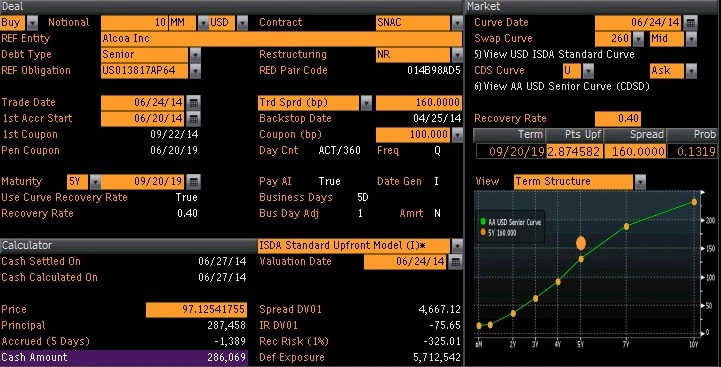
\includegraphics[width=6.3in, height=3.8in]{images/AlcoaIncCDS.jpg}
\caption{This is a Bloomberg screenshot that shows the details of an actual CDS transaction on Alcoa Inc priced on June 24, 2014 with 5 years of maturity. The screenshot consists of three sections: the Deal section (upperleft), Calculator section (bottomleft), and Market section (right side). The Deal section is where traders mostly input detailed information of the trade, such as \textbf{trade date} and \textbf{coupon}. The Calculator section shows the calculation results of the CDS contract after the trader has entered the trade information in Deal section. Traders rely on these calculation results to make decisions on trades. The Market section shows information of the relevant market rates (such as LIBOR) that we concern as discount factors. This include \textbf{recovery rate} and \textbf{default probability}.}
\label{AlcoaIncCDS}
\end{figure}

\subsection{Deal Section}

\begin{figure}[H]
\centering
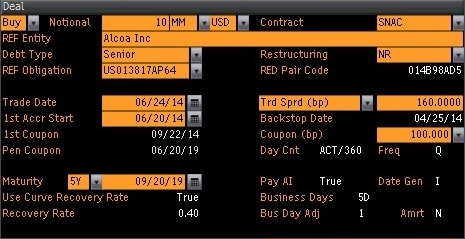
\includegraphics[width=6.3in, height=3.8in]{images/AlcoaIncCDSDeal.jpg}
\caption{This is a figure of Deal section cropped from Figure 2. Traders enter most of the CDS trade information in Deal section, and Calculation section and Market section rely heavily on information provided in ``Deal'' section. Familiar terms are \textbf{notional amount}, \textbf{trade date},\textbf{trade spread}, and \textbf{coupon}. Recall that trade spread is the coupon traders \textit{would} have traded at before Big Bang Protocol standardized the coupon rate. \textbf{Maturity} means how long the protection contract lasts and when the coverage finishes. Here, the first slot ``5Y'' means the contract lasts 5 years, and second slot means that the contract will end on Sept. 20, 2019.}
\label{deal}
\end{figure}

In Deal section, \textbf{REF Entity} (Reference Entity) refers to the name of the company (Alcoa, in this case) and \textbf{RED Pair Code} is a Markit product that stands for Reference Entity Database. Each entity/seniority pair has a unique six-digit RED Pair Code that matches the first six digits of the nine-digit RED Pair Code, and a ``preferred reference obligation,'' which is the default reference obligation for CDS  trades. A user can input either the six-digit RED Pair Code or the nine-digit RED Pair Code. The input ``014B98'' is the six-digit RED Pair Code for ``Alcoa''. The label \textbf{Debt type}, marked as ``Senior,'' refers to the seniority of the debt. The \textbf{REF Obligation} (Reference Obligation) refers to the bond involved in the CDS, and it matches the ISIN. The label \textbf{Restructuring} refers to which term of debt restructuring we agree on: For example, U.S. traders usually do not accept debt restructuring as CDS payment, and debt restructuring is often considered as bankcrupcy. Therefore, when trading CDS in U.S., we usually specify Restructuring to ``NR,'' which stands for ``No Restructuring.'' In Europe, however, traders usually consider certain types of debt restructuring acceptable and different from bankcrupcy, so European traders usually specify Restructuring to ``MMR'' which stands for Modified ``Modified Restructuring''. 

At the top left, we see the CDS contract type is \textbf{SNAC} (\textbf{Standard North American Contract}), which is a convention that specifies how North American single-name CDS are supposed to trade. In European markets, CDS belong to the \textbf{STEC} category, or Standard European Contract.

At the lower right, we see \textbf{Maturity} has two slots. The first slot is the \textbf{tenor}, or length, of the contract. This means that the buyer is protected for 5 years in this case. Tenor can also be denoted in months, e.g. ``5M''. The second slot is \textbf{Maturity Date}, or \textbf{end date}, of the contract. This refers to when the protection is over. 

On the right side, \textbf{Trd Sprd (bp)} is just \textbf{spread}. Recall that spread is the ``coupon'' that we \textit{trade} on before the Big Bang Protocol. Here the spread is equal to 160 basis points, but notice that spread can also be denoted in percentage. \textbf{Coupon (bp)} refers to \textbf{coupon} in basis points, which is equal to 100 basis points here. The protection buyer will have to make an upfront payment to account for the extra 60 basis points paid quarterly (15 bp per quarter) over a period of five years.

At the lower left, \textbf{Recovery Rate} is set to 0.40 and we use \textbf{Curve Recovery Rate} by default. On the bottom right, \textbf{trading conventions} are listed. For example, \textbf{Day Convention} (``Day Cnt'') denotes what type of convention of dates we follow in this trading. Here, ACT/360 means that we assume there are 360 days in a year. 

On the left, \textbf{Trade Date} is the date when we trade CDS; \textbf{First Accrual Start Date} (``1st Accr Start'') is the previous \textbf{roll date} adjusted for weekdays before the Trade Date; \textbf{First Coupon Payment Date} (``1st Coupon'') is the date when first coupon payment are paid. This is the first roll date adjusted for weekdays after our trade date. \textbf{Penultimate Coupon Payment Date} (``Pen Coupon'') is the second last date when we pay our coupon payment. It is the weekday-adjusted roll date before the maturity date. Notice that the maturity date must \textbf{not} be adjusted, while other dates must be adjusted for businessdays. In other words, maturity dates can be on non-business days, but other dates cannot.

\newpage
\subsection{Calculator Section}
\label{Calculator section}
\begin{figure}[H]
\centering
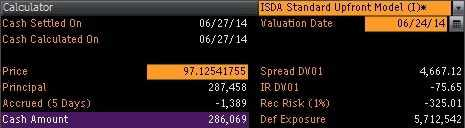
\includegraphics[width=5.5in, height=2.5in]{images/AlcoaIncCDSCalculator.jpg}
\caption{
This figure is the Calculation section cropped from Figure 2. We can see here that we are using ISDA Standard Upfront Model for the CDS pricing, and the valuation is done on the trade date while cash settlement date is three days after. Calculation section takes in the information entered by traders in Deal section and calculate some important results,  such as \textbf{CDS price}, \textbf{principle amount}, and \textbf{cash amount}. Here, cash amount is the same as \textbf{upfront payment} ($U$). Traders use these calculation results to make trading decisions and risk management.}
\label{AlcoaIncCDSCalculator}
\end{figure}

At the top left, we choose \textbf{ISDA Standard Upfront Model} to calculate CDS pricing. \textbf{Principal}, or the mark-to-market value, of this contract is \$287458. This amount is the sum of the expected present value of each coupon payment. If we account for the accrued amount which the protection buyer does not have to pay, the upfront value is \$286069. 

The ISDA protocol, since April 2009, specifies that all premium payments, by default, start on the roll date before the Trade Date. So if the Trade Date is June 24, 2014, the \textbf{Accrual Begin Date} is, by default, June 20, 2014. Now if the Accrual Begin Date is 4 days before the Trade Date, protection buyers would not want (and are not obligated) to pay interest for the 5 days they have not received protection for. \textbf{Accrued interest} can be calculated using the equation below:

\begin{equation}
 \begin{aligned}
  {\rm Accrued = \frac{5}{360} \times \frac{1}{100} \times \$10000000 = \$1,389}
    \end{aligned}
\end{equation}

Now let's focus on the labels at the lower right: Spread DV01, IR DV01, Recovery Risk (1\%), and Default Exposure. These four parameters indicate the change of upfront if small adjustments are made to the trade. For example, Spread DV01 measures how much upfront payment would change if spread was set a little higher. However, to understand these four concepts, we have to introduce \textbf{PV01} first.

\subsubsection{PV01}
\label{sec:PV01}

\textbf{PV01} stands for ``Present Value 01'', which is the present value of a stream of 1 basis points of payments. We can also use the formula below to calculate the principal amount (clean upfront payment) with PV01:

\begin{equation}
 \begin{aligned}
  Principal = |Coupon - Spread| \times PV01 \times Notional
    \end{aligned}
\end{equation}

PV01 can also be used to calculate the cash flows and risk measures of a CDS. It is sometimes referred to as the \textbf{CDS duration} or \textbf{risky duration}. Analytically, PV01 can be calculated by

\begin{displaymath}
PV01 =  \sum_tDf(t_i)S(t_i)B(t_i), \nonumber\\
\end{displaymath}
\begin{itemize}
\item $i =$ coupon index,
\item $t_i =$ coupon date: date on which coupon payments are made
\item $B(t_i) =$ day count fraction at $t_i$: fraction of the day on which the coupon payment is made upon, such as 360 or 365, depending on the day count convention of the CDS
\item $Df(f_i) =$ discount factor until $t_i$,
\item $S(t_i) =$ survival probability until $t_i$,
\end{itemize}

\subsubsection{Spread DV01}
\label{sec:spread.DV.01}

\textbf{Spread DV01} (also known as \textbf{Sprd DV01}, \textbf{Credit DV01}, \textbf{Spread Delta}, \textbf{DV01}) stands for ``Spread Dollar Value 01.'' It measures the change of upfront payment if spread increases by 1, and reflects the sensitivity of a CDS contract mark-to-market to a parallel shift in the term structure of the par spread. In other words, it reflects the risk duration of a CDS trade. 

DV01 should always be positive for a protection buyer since she is short credit, and a rising spread is a sign of credit deterioration. Starting with PV01 and taking the derivative with respect to the spread gives us:

\begin{align*}
  PV &= (S - C) \times PV01 \\
  DV01 &= \frac{\partial PV}{\partial S} \\
  &= PV01 + (S - C) \frac{\partial PV01}{\partial S},
\end{align*}

where $S$ is the spread of the contract and $C$ is the coupon. Both DV01 and PV01 are measured in dollars and are equal if the spread equals the coupon.

\subsubsection{IR DV01}
\label{sec:IRDV01}
\textbf{IR DV01} stands for ``Interest Rate Dollar Value 01.'' It measures the change in value of a CDS contract for a 1 bp parallel increase in the interest rate curve. IR DV01 is, typically, a much smaller dollar value than Spread DV01 because moves in overall interest rates have a much smaller effect on the value of a CDS contract than does a move in the CDS spread itself. Formula given below.

\begin{align*}
  \text{IR DV01} &= 0.0001 \frac{\partial PV}{\partial r} = 0.0001 (S - C) \times \frac{\partial PV01}{\partial r}
\end{align*}

A multiple of $0.0001$ appears in the formula, because we are calculating the change of upfront payment with a 1 bp increase in the interest rate.

\subsubsection{Rec Risk (1\%)}
\textbf{Rec Risk (1\%)} stands for ``Recovery Risk 1\%.'' It measures the change of upfront payment if the recovery risk increases by 1\%. Formula given below.

\begin{align*}
  \text{Rec Risk (1\%)} &= 0.01 \frac{\partial PV}{\partial RR} = 0.01 (S - C) \times \frac{\partial PV01}{\partial RR}
\end{align*}

A multiple of $0.01$ appears in the formula, because we are calculating the change of upfront payment with a $1\%$ increase in the recovery rate.

\subsubsection{Default Exposure}
\label{sec:DefaultExpo}

Default Exposure refers to the expoure to default of a CDS contract. It can be calculated with Recovery Rate, Notional Amount, and Principal as below:

\begin{equation}
  \text{Default Exposure} = (1 - \text{Recovery Rate}) \times \text{Notional}
  - \text{Principal}. \nonumber
\end{equation} 

\subsection{Market Section}
\label{Market section}
\begin{figure}[H]
\centering
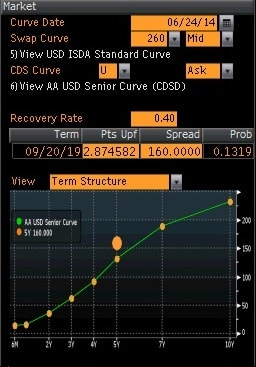
\includegraphics[width=3in, height=4.5in]{images/AlcoaIncCDSMarket.jpg}
\caption{
This figure is the ``Market'' section cropped from Figure 2. Market section is another field where traders views information of market curve rates and CDS term structure. \textbf{Curve Date} is the date of LIBOR rates we use to price CDS (see below for important clarifications). \textbf{Recovery rate} is the percent of a equity's value that can be recovered. \textbf{Points upfront} refers to the upfront payment as a percentage of the notional amount. \textbf{Spread} is the coupon rate we \textit{would} have traded at before Big Bang Protocol standardized coupon rate. \textbf{Default probability} (or probability of default) is the risk-neutral probability of default that makes equal the potential cash flows from both buy and sell side of the CDS.}

\label{AlcoaIncCDSMarket}
\end{figure}

\subsubsection{Curve Date}
\textbf{Curve date} is the date of interest rate we use to price CDS. As we recall, the trade date of this CDS trading is Jun. 24, 2014, and we see the Curve Date is also Jun. 24, 2014. However, this does not mean that we actually use the interest rates on Jun. 24, 2014; we are actually using interest rates on Jun. 23, 2014. For CDS pricing, we use the interest rates on the day before the trade date. And if the day before trade date is not a business day, we adjust to the nearest business day before. Therefore, if the trade date is Jun. 24, 2014, then we will use interest rates on Jun. 23, 2014 (Monday). If the trade date is Jun. 23, 2014, then we will use interest rates on Jun. 20, 2014 (Friday), since Jun. 22 is a Sunday. In Bloomberg Terminal, this adjustment is already taken into account, so the Curve Date on screen shows Jun. 24 while we are actually using interest rates on Jun. 23.
\\
\subsubsection{Default Probability}
\label{sec:DefaultProb}

As we did in the two-period case, we also have to account for the probability of default for each period. The probability of a company defaulting is different across time period, and we assume the probability is constant within a specific time period. The term structure of these probabilities are known as the \textbf{hazard rates} and the hazard rate function is piecewise constant.  

The probability of a company surviving till the end of period \textit{n} is the probability that it survives period \textit{n}, conditional on it having survived the previous \textit{n-1} periods. This is known as the \textbf{survival probability}. The survival probability function can be equated with the \textbf{hazard rates} function or the distribution of the company's risk-neutral probability of default as below,

\begin{displaymath}
S_t = 1 - Q_t = 1 - \int_0^T q_t dt\, \nonumber\\
\end{displaymath}

Here on the screenshot, the ``prob'' label refers to \textbf{default probability}. Recall in the simple one-period case, the default probability can be calculated as below:

\label{eqn:recovery}
\begin{align}
  \rm Portfolio\hspace{3pt}manager's\hspace{3pt}expected\hspace{3pt}cash\hspace{3pt}flows &= \rm JPM's\hspace{3pt}expected\hspace{3pt}cash\hspace{3pt}flows \\
  \rm - C + (P \times V \times (1 - RR)) &= C - (P \times V \times (1 - RR))
\end{align}

where $RR$ refers to the recovery rate and, as before, $P$ is the risk-neutral probability of default, $C$ is the coupon payment, and $V$ is the notional value. However, in reality the non-default probability in a certain time-period, say from $t_i$ to $t_j$, decays exponentially with multiplier determined by the current spread at time $t$, time $t$ itself, and the recovery rate. In other words, the default probability is non-constant but can be mathematically expressed as below:

\begin{equation}
  \text{Non-Default Probability} \approx e ^ {\frac{rt}{1-R}}, 
\end{equation}

So the default probability at time $t$ is:

\begin{equation}
  \text{Default Probability} \approx 1 - e ^ {\frac{rt}{1-R}}, \nonumber
\end{equation}

where $r$ is the spread, $t$ is the time to maturity, and $R$ is the recovery rate. 

\subsubsection{Term Structure}

A CDS term structure is similar to the interest rate curve in that it has the fair spreads of CDS contracts with different maturities. For liquid reference names, these rates are easily available. If the CDS is not liquid, we can use the underlying bond's price to determine the hazard rates. However, if there are only a couple of maturity dates available, we can assume a flat CDS curve. \textbf{Term structure} is shown in Market section (X-axis is maturity and Y-axis is spread). The green line with little yellow dots is the ``AA USD Senior Curve'', which means we are buying senior debt protection in USD of Alcoa Inc (stock symbol AA). The big yellow dot is the CDS contract we buy, here at 5-year maturity and 160 basis points of spread.

\newpage

\subsection{Markit CDS Calculator Overview}
\label{Markit}

\begin{figure}[H]
\centering
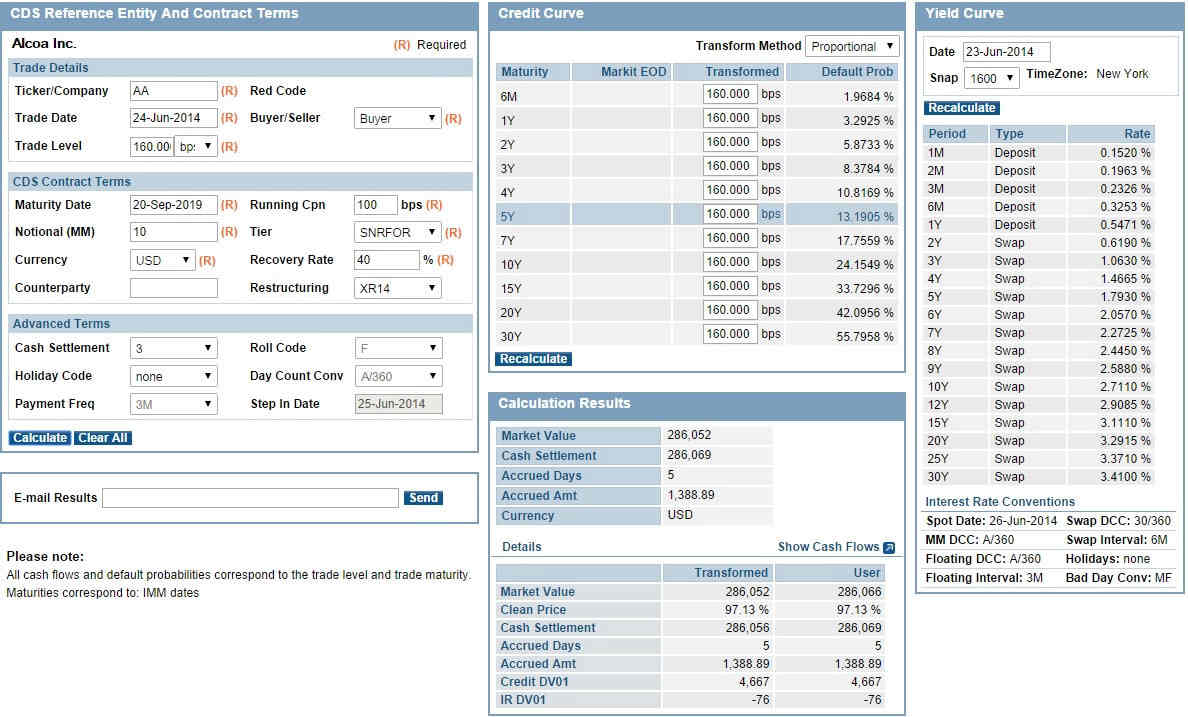
\includegraphics[width=6.3in, height=4.8in]{images/MarkitCDSAlcoa.jpg}
\caption{
This is a screenshot of the online Markit CDS Calculator. It shows the same trade as the above Bloomberg screenshot: a purhcase of senior debt protection of Alcoa Inc with a tenor of five years on Jun. 24, 2014. The layout is divided into four sections: Contract section (left), Credit Curve section (center up), Calculation section (center down), and Yield Curve section (right). In Contract section, the fields are similar to those in Deal section in Bloomberg, except that we have to manually set holiday code (in Bloomberg this is automatically set according to users' input). Credit Curve section shows the term structure in a table, while in Bloomberg term structure is shown in a graph. Notice that we have the advantage of viewing default probabilities at different maturities in Markit, but advantage of viewing different spread levels in Bloomberg. our contract choice is highlighted in blue. The Calculation section is very similar to that in Bloomberg, with small differences explained below. The Yield Curve section shows the LIBOR rates (discount factor) we use, and notice that curve date is adjusted here.
}
\end{figure}

\subsubsection{Terminology Differences}
On the upper left, \textbf{Trade Level} means the same as \textbf{spread}. We can present spread in either basis points (``bp'') or percentages. In ``CDS Contract Terms,'' \textbf{Running Cpn} just means \textbf{coupon}. In ``Advanced Terms,'' \textbf{Holiday Code} refers to the holiday convention we are using. As we recall, CDS trading in JPY follows a different holiday convention than in other currencies. Therefore, we can select either ``none'' or ``JPY'' for ``Holiday Code.''

In ``Calculation Results,'' \textbf{Cash Settlement} is the same as \textbf{Cash Amount} in Bloomberg, \textbf{Clean Price} is same as \textbf{Price}, the \textbf{Accured Amount} in Markit and Bloomberg has different signs (one is positive while the other negative), and \textbf{Credit DV01} is the same as \textbf{Spread DV01}.

\subsubsection{Yield Curve Section and Discount Factor}

In the actual CDS world we would have to discount each of the 15 bp payments by the interest rates that apply for the same maturity. This is known as the discount factor. In the risk-neutral valuation framework, the risk free curve is the discount factor used in the calculation of the present value of CDS. In calculating the price of a CDS, we use the swap curve of the \textit{previous day} (this will be further explained later in ``Curve Date'' section), and use the rates for the corresponding currency. So for CDS denominated in USD, we will use the US treasury rates, and for those in GBP we will use UK Government bond yields, and so on. If we look at Figure \ref{fig:AlcoaRates}, we can see the yields for different treasury bonds at 4pm EST on June 23, 2014, which will be used for pricing the CDS of Alcoa.

The Yield Curve section in the above figure shows the risk-free rates with their day count conventions on June 23, 2014 at 4pm EST. These are the rates that will be used to price the CDS of Alcoa on June 24, 2014. \textbf{MM DCC}, \textbf{Floating DCC} and \textbf{Swap DCC} refer to the Day Count Conventions being used to calculate the different kinds of rates. A \textbf{Swap Interval} of `6M' implies that interest is paid every six months or semi-annually. These conventions are different for each currency.


\subsubsection{Risky Discount Factor}

Together, the discount factor and the survival probability are known as the \textbf{risky discount factor}. The discount factor is used in calculating the upfront value for a CDS maturing over \textit{n} periods. Therefore the principal or mark-to-market value can be calculated using the formula below:

\begin{equation}
 \begin{aligned}
   \displaystyle\sum_{i=1}^{n}|Coupon - Spread| \times (1-q(t)) \times D(0, t(i))
    \end{aligned}
\end{equation}

\subsection{CDS Indices}
\label{sec:CDSIndices}

Holding a disproportionate number of Alcoa bonds in a portfolio is naturally a risky idea. Successful portfolio managers prefer to distribute their risk by holding a portfolio with hundreds, if not thousands, of different positions. 

Instead of holding Alcoa bonds with a face value of \$10 million, say our portfolio manager decides to take on less risk by holding bonds of 100 different IG companies. This is known as \textbf{diversification}. Although this strategy reduces her exposure to the credit risk of any particular company, she hasn't reduced her exposure to factors that might affect a wide variety of assets simulatenously, such as interest rate risk or political risk. Fortunately, in the modern financial world, she has the option of purchasing multi-name CDS, or CDS indices, which contain a basket of CDS. The two most common indices are CDX and iTraxx, which represent North American CDS and European CDS, respectively.
 
Moreover, if our portfolio manager has a high-risk appetite and wants to earn a higher return for her investors, she may invest a portion of her portfolio in bonds that have a lower credit rating but provide a higher yield. She may hedge this position by investing in a tranche of CDS indices such as the North American High Yield CDS index, which specifially offers protection on high yield bonds of 100 different companies. CDX and iTraxx are broken into smaller CDS based on sectors such as automobiles or consumer goods.

These index products trade in high volumes and are very liquid. In this vignette, we only discuss the pricing mechanisms of single-name CDS and do not delve into the more complex world of multi-name CDS. However, it is important to understand their relevance as most CDS contracts involve companies in these indices.

\newpage
\section{Using the CDS Package}
\label{CDSpkg}

In this section, we will demonstrate the use of the \textbf{CDS} package in detail and provide a series of examples. The \textbf{CDS} package implements the Standard Model, allowing users to value credit default swaps and calculate various risk measures associated with these instruments. 

\subsection{ISDA Standard Model}
\label{sec:ISDAStMod}

The ISDA has created the ``Standard Model,'' which allows market participants to calculate cash settlement from conventional spread quotations, convert between conventional spread and upfront payments, and build the spread curve of a CDS. 

The Standard Model allows market participants to convert between the par spread and the upfront payment, and compute the cash settlement amount for a standard contract.

The ISDA also standardizes the interest rates used by the Standard Model in valuing a CDS contract. There are two types of rates used in valuing a USD-denominated CDS contract: cash rates and swap rates. Cash rates are of the following maturities: one, two, three, and six month(s), and one year. These refer to the yields of zero-coupon bonds that have a maturity of less than one year; US treasuries with a maturity of one year or less are zero-coupon bonds. They are provided by the British Bankers' Association (BBA). Swap rates, or yields of coupon bond siwht a maturity of over one year, are of maturity 2, 3, 4, 5, 6, 7, 8, 9, 10, 12, 15, 20, 25, and 30 years, and are provided by ICAP \citep{rates}. The Standard Model follows the conventions below for interpolation of the entire USD yield curve:
\begin{itemize}
\item The day count convention (DCC) for money market instruments and
  the floating legs of the swaps is \textbf{ACT/360}.
\item DCC for floating legs of the swaps is \textbf{30/360}.
\item Payment frequency for fixed legs of the swaps is 6 months.
\item Payment frequency for floating legs of the swaps is 3
  months.\footnote{See
    \url{http://www.fincad.com/derivatives-resources/wiki/swap-pricing.aspx}
    for details on floating and fixed legs calculation.}
\item A business day calendar of weekdays (Monday to Friday) is
  assumed. Saturdays and Sundays will be the only non-business days.
\item If a date falls on a non-business day, the convention used for
  adjusting coupon payment dates is \textbf{M} (Modified Following).
\item Recovery Rate is the estimated percentage of par value that
  bondholders will receive after a credit event. It is commonly
  reported in percentage of notional value. CDS contracts for corporate bonds
  assume a 40\% recovery rate for valuation purposes. 
\end{itemize}


Currently, a market participant can conduct CDS-related calculations by using the \textbf{CDSW Calculator} on a Bloomberg Terminal or the Markit CDS Calculator\footnote{The Markit CDS Calculator is available
  at \url{http://www.markit.com/markit.jsp?jsppage=pv.jsp}.}. The \textbf{CDS} package provides tools for valuing a single-name CDS contract. The default setting allows a user to value a USD-denominated CDS contract following the Standard Model as mentioned before. She can also specify her own set of parameters to customize the calculation. 

\subsection{CDS Class}
\label{class:CDS}

In the \textbf{CDS} package, we call the function \texttt{CDS} to construct an object of a class \texttt{CDS}. Below we show an example of how to construct a CDS contract in the package.

\begin{Schunk}
\begin{Sinput}
> library(CDS)
> cds1 <- CDS(name     = "Alcoa",
+             RED      = "49EB20",
+             date     = as.Date("2014-06-24"),
+             tenor    = 5,
+             notional = 1e7,
+             coupon   = 100,
+             spread   = 160)
\end{Sinput}
\end{Schunk}

Here the user enters the CDS contract with ``Alcoa'' as the underlying entity and sets the spread at 160 bps and the coupon at 100 bps. However, the valuation of a CDS contract requires neither the Reference Entity nor the RED Code. She does not have to know that information to use the \textbf{CDS} package. As shown below, as long as she inputs the same \texttt{date}, \texttt{spread}, and \texttt{maturity} information, the valuation of the contract will be the same.

\begin{Schunk}
\begin{Sinput}
> library(CDS)
> cds2 <- CDS(date     = as.Date("2014-06-24"),
+             maturity = as.Date("2019-06-20"),
+             spread   = 160)
\end{Sinput}
\end{Schunk}

\subsection{Generic Methods}
\label{sec:GenericMethods}

\subsubsection{summary Method}
\label{sec:SummaryFunction}

A user can call \texttt{summary} on a \texttt{cds1} to view essential information on the contract.

\begin{Schunk}
\begin{Sinput}
> summary(cds1)
\end{Sinput}
\begin{Soutput}
Contract Type:                      SNAC   Date:                      2014-06-24
Entity Name:                       Alcoa   RED:                           49EB20
Currency:                            USD   End Date:                  2019-09-20
Spread:                              160   Coupon:                           100
Upfront:                         286,069   Spread DV01:                    4,667
IR DV01:                          -75.64   Rec Risk (1 pct):             -330.19
\end{Soutput}
\end{Schunk}

In the summary output, it shows that the type of the CDS contract is ``SNAC''. This means that the CDS contract follows the Standard North American Corporate (SNAC) CDS Contract specifications.\footnote{See \url{http://www.cdsmodel.com/assets/cds-model/docs/Standard\%20CDS\%20Contract\%20Specification.pdf} for details.}  \texttt{Date} refers to the trade date which, in this example, is June 24, 2014. \texttt{Entity Name} refers to the entity name of the CDS contract which, in this example, is ``Alcoa''. The \texttt{RED} code is ``48EB20'' as specified by the user. \texttt{currency} (``USD'' in this case) is the currency of the CDS contract with three options of ``USD'', ``JPY'' and ``EUR''. \texttt{End Date} is the same as maturity and is the date on which the CDS contract expires. Recall from previous sections that \texttt{End Date} can only fall on one of the four standard dates. In our example, the \texttt{End Date} is ``2019-09-20''. \texttt{spread} shows that the quoted spread for the contract is 160 bps and the coupon is 100 bps as shown in the \texttt{Coupon} field. \texttt{Upfront} indicates the dirty upfront payment in dollars or the cash settlement amount which, in this example, is \$286,069.

The remaining three items from the \texttt{summary} output  are \texttt{Spread DV01}, \texttt{IR DV01}, and \texttt{Rec Risk (1 pct)}. Spread DV01 is the increase in the upfront value when the spread increase by one basis point. In \texttt{cds1}, the Spread DV01 is \$4,667. IR DV01 is the increase in the upfront value when the interest rate on all maturities of the interest curve increase by a single basis point which, in our example, is \$-75.64. Rec Risk (1 pct) is the increase in the upfront value when the recovery rate increase by one percentage point. In \texttt{cds1}, the Rec Risk (1 pct) is \$-330.19.

Besides calling the \texttt{summary} method, one can type in the name of the \texttt{CDS} class object in the current \textbf{R} Session and obtain a full description of the CDS contract.

\subsubsection{Show Method}
\label{sec:showMethod}

\begin{Schunk}
\begin{Sinput}
> cds1
\end{Sinput}
\begin{Soutput}
CDS Contract 
Contract Type:                      SNAC   Currency:                         USD
Entity Name:                       Alcoa   RED:                           49EB20
date:                         2014-06-24

Calculation 
price:                             97.13   Spread:                           160
Principal:                       287,458   Spread DV01:                    4,667
Accrual:                          -1,389   IR DV01:                       -75.64
Upfront:                         286,069   Rec Risk (1 pct):             -330.19
Default Prob:                     0.1322
\end{Soutput}
\end{Schunk}

\subsection{CDS Pricing Related Functions}
\label{sec:CDSpricingFunctions}

\subsubsection{CS10}
\label{sec:CS10}

\texttt{``CS10''} is a method which calculates the change in value of the CDS contract when the spread of the contract increases by 10\%. \texttt{CS10} takes in a \texttt{CDS} class object formed by calling the \texttt{CDS} function. The CS10 of \texttt{cds1} is \$25385.2. Or you can calculate CS10 by inputing a dataframe. 

\begin{Schunk}
\begin{Sinput}
> x <- data.frame(date = as.Date(c("2014-04-22", "2014-04-22")),
+                 currency = c("USD", "EUR"),
+                 tenor = c(5, 5),
+                 spread = c(120, 110),
+                 coupon = c(100, 100),
+                 recovery = c(0.4, 0.4),
+                 notional = c(1e7, 1e7),
+                 stringsAsFactors = FALSE)
> CS10(x)
\end{Sinput}
\begin{Soutput}
[1] 56952.65 53430.42
\end{Soutput}
\end{Schunk}

\subsubsection{``get.rates'' Function}
\label{sec:get.ratesFunction}

This is a function used to obtain the interest rate curve for a given currency on a given date, along with the day count convention for that currency.

\begin{Schunk}
\begin{Sinput}
> cds1.rates <- get.rates(date = as.Date("2014-06-24"), currency = "USD")
\end{Sinput}
\end{Schunk}

The output from the get.rates function is a data frame which contains rates of various expiries. They are directly fetched from a local data frame called \texttt{rates.RData}, or, if the requested date is not available in \texttt{rates.RData}, obtained from the Markit website based on the specifications \citep{rates}.

\begin{Schunk}
\begin{Sinput}
> cds1.rates
\end{Sinput}
\begin{Soutput}
            date currency expiry     rate type
61418 2014-06-24      USD     1M 0.001520    M
61419 2014-06-24      USD     2M 0.001963    M
61420 2014-06-24      USD     3M 0.002326    M
61421 2014-06-24      USD     6M 0.003253    M
61422 2014-06-24      USD     1Y 0.005471    M
61423 2014-06-24      USD     2Y 0.006190    S
61424 2014-06-24      USD     3Y 0.010630    S
61425 2014-06-24      USD     4Y 0.014665    S
61426 2014-06-24      USD     5Y 0.017930    S
61427 2014-06-24      USD     6Y 0.020570    S
61428 2014-06-24      USD     7Y 0.022725    S
61429 2014-06-24      USD     8Y 0.024450    S
61430 2014-06-24      USD     9Y 0.025880    S
61431 2014-06-24      USD    10Y 0.027110    S
61432 2014-06-24      USD    12Y 0.029085    S
61433 2014-06-24      USD    15Y 0.031110    S
61434 2014-06-24      USD    20Y 0.032915    S
61435 2014-06-24      USD    25Y 0.033710    S
61436 2014-06-24      USD    30Y 0.034100    S
\end{Soutput}
\end{Schunk}

\subsection{Risk Related Functions}
\label{sec:riskFunctions}

\subsubsection{``rec.risk.01'' Function}

\texttt{rec.risk.01} is a function which takes a data frame of date, currency, tenor (or maturity), spread, coupon, recovery and notional and calculates the rec.risk.01 values for each row. Recall that \textbf{Rec Risk (1\%)} stands for ``Recovery Risk 1\%.'' It measures the change of upfront payment if the recovery risk increases by 1\%. Formula given below.

\begin{align*}
  \text{Rec Risk (1\%)} &= 0.01 \frac{\partial PV}{\partial RR} = 0.01 (S - C) \times \frac{\partial PV01}{\partial RR}
\end{align*}

\begin{Schunk}
\begin{Sinput}
> rec.risk.01(data.frame(date     = as.Date("2014-06-24"),
+                        currency = "USD",
+                        tenor    = 5,
+                        spread   = 160,
+                        coupon   = 100,
+                        recovery = 0.4,
+                        notional = 1e7))
\end{Sinput}
\begin{Soutput}
[1] -330.1858
\end{Soutput}
\end{Schunk}

\subsubsection{``IR.DV01'' Function}

\texttt{IR.DV01} is a function which takes a data frame of date, currency, tenor (or maturity), spread, coupon, recovery and notional and calculates the IR.DV01 values for each row.

Recall that \textbf{IR DV01} stands for ``Interest Rate Dollar Value 01.'' It measures the change in value of a CDS contract for a 1 bp parallel increase in the interest rate curve. Formula given below.

\begin{align*}
  \text{IR DV01} &= 0.0001 \frac{\partial PV}{\partial r} = 0.0001 (S - C) \times \frac{\partial PV01}{\partial r}
\end{align*}


\begin{Schunk}
\begin{Sinput}
> IR.DV01(data.frame(date     = as.Date("2014-04-22"),
+                    currency = "USD",
+                    tenor    = 5,
+                    spread   = 160,
+                    coupon   = 100,
+                    recovery = 0.4,
+                    notional = 1e7))
\end{Sinput}
\begin{Soutput}
[1] -73.72284
\end{Soutput}
\end{Schunk}


\subsubsection{``spread.DV01'' Function}

\texttt{spread.DV01} is a function which takes a data frame of date, currency, tenor (or maturity), spread, coupon, recovery and notional and calculates the spread.DV01 values for each row.

Recall that \textbf{Spread DV01} stands for ``Spread Dollar Value 01.'' It measures the risk duration of a CDS trade. 

\begin{align*}
  PV &= (S - C) \times PV01 \\
  DV01 &= \frac{\partial PV}{\partial S} \\
  &= PV01 + (S - C) \frac{\partial PV01}{\partial S},
\end{align*}

\begin{Schunk}
\begin{Sinput}
> spread.DV01(data.frame(date     = as.Date("2014-04-22"),
+                        currency = "USD",
+                        tenor    = 5,
+                        spread   = 160,
+                        coupon   = 100,
+                        recovery = 0.4,
+                        notional = 1e7))
\end{Sinput}
\begin{Soutput}
[1] 4610.056
\end{Soutput}
\end{Schunk}


\subsubsection{``spread.to.pd'' Function}

\texttt{spread.to.pd} is a function which calculates the probability of default using the model provided in the Bloomberg manual. It also takes data frame input.

\begin{Schunk}
\begin{Sinput}
> spread.to.pd(data.frame(date     = Sys.Date(),
+                         spread   = 160,
+                         tenor    = 5,
+                         recovery = 0.4,
+                         currency = "USD"))
\end{Sinput}
\begin{Soutput}
[1] 0.1291594
\end{Soutput}
\end{Schunk}

\section{Conclusion}

\newpage
\bibliography{CDS}
\cite{barclays}
\cite{bloomberg}
\cite{openGamma}
\cite{glossary}
\cite{cdsOrigins}
\cite{blythe}
\cite{jk}
\cite{rates}
\cite{kane:david}
\cite{creditDerivatives}
\end{document}

%% Consider the following example: there exists a portfolio manager---a manager of multiple investments---who has just bought \$100,000 worth of bonds from company X. We'll discuss what a bond is in a later section, but for now just think of it as an I.O.U.; the portfolio manager lends \$100,000 to company X for a certain time period, and at the end of the period, company X returns the \$100,000 to the manager. After she buys the bonds, however, her confidence in company X's ability to make good on its obligation and return the \$100,000 begins to waiver. What should she do? 

%% One popular option in today's economy is to enter a \textbf{credit default swap} (CDS) agreement with a third party. In this case, the portfolio manager could enter a CDS contract in which she pays a fee to the third party, and if company X can't pay back the sum of \$100,000, the third party will pay the remaining monetary amount. In other words, the portfolio manager pays a fee in exchange for protection against company X's inability to meet its obligation. 


%The cash flows from the protection  buyer to the seller, when there is no credit event, would look like Figure \ref{fig:CDSnoevent}
